% -----------------------------------
% -----------------------------------
% abnTeX2: Normas ABNT NBR 14724:2011 + sugestões FGV/EMAp. 

% Autor: Lauro César Araujo
% Adaptações EMAp: Lucas Machado Moschen 
% Copyright 2012-2018 by abnTeX2 group at http://www.abntex.net.br/ 

%% This work may be distributed and/or modified under the
%% conditions of the LaTeX Project Public License, either version 1.3
%% of this license or (at your option) any later version.
%% The latest version of this license is in
%%   http://www.latex-project.org/lppl.txt
%% and version 1.3 or later is part of all distributions of LaTeX
%% version 2005/12/01 or later.
% ----------------------------------
% ----------------------------------
\documentclass[
	% -- opções da classe memoir --
	12pt,				% tamanho da fonte
	%openright,			% capítulos começam em página ímpar (insere página vazia caso preciso)
	oneside,			% para impressão em recto e verso. Oposto a oneside
	a4paper,			% tamanho do papel. 
	% -- opções da classe abntex2 --
	%chapter=TITLE,		% títulos de capítulos convertidos em letras maiúsculas
	%section=TITLE,		% títulos de seções convertidos em letras maiúsculas
	%subsection=TITLE,	% títulos de subseções convertidos em letras maiúsculas
	%subsubsection=TITLE,% títulos de subsubseções convertidos em letras maiúsculas
	% -- opções do pacote babel --
	english,			% idioma para inglês
	%brazil				% idioma para português
	]{abntex2}

%------------------------------------------------
%-------------- Pacotes necessários -------------
%------------------------------------------------

% Escrita 
\usepackage[T1]{fontenc}
\usepackage[utf8]{inputenc}
\usepackage{lmodern}
\usepackage{microtype} % para melhorias de justificação
\usepackage{indentfirst}
\usepackage{csquotes}

\renewcommand{\ABNTEXchapterfont}{\fontfamily{ptm}\fontseries{b}\selectfont}

% Gráficos 
\usepackage{color}
\usepackage{caption}
\usepackage{subcaption}
\usepackage{multirow}
\usepackage{graphicx}
\usepackage{pdfpages}
\graphicspath{{../../images/}}

% Matemáticos 
\usepackage{bbm}
\usepackage{amsthm, amssymb, amsmath, mathtools}

% Outros 
\usepackage{lipsum}
%\usepackage[textsize=tiny, textwidth=15mm]{todonotes}
\usepackage{multirow}
\usepackage{listings}
\usepackage{lstbayes}

% Citações 
%\usepackage[brazilian,hyperpageref]{backref}
%\usepackage[alf]{abntex2cite}	% Citações padrão ABNT
\usepackage[style=abnt]{biblatex}
\addbibresource{biblio.bib}  

% \renewcommand{\backrefpagesname}{Citado na(s) página(s):~}
% % Texto padrão antes do número das páginas
% \renewcommand{\backref}{}
% % Define os textos da citação
% \renewcommand*{\backrefalt}[4]{
% 	\ifcase #1 %
% 		Nenhuma citação no texto.%
% 	\or
% 		Citado na página #2.%
% 	\else
% 		Citado #1 vezes nas páginas #2.%
% 	\fi}%
% ---

%----------------------------------------
%------- Capa e Folha de Rosto ----------
%----------------------------------------

\newcommand{\subtitulo}[1]{\title{#1}}
\newcommand{\imprimirsubtitulo}{\thetitle}

\renewcommand{\imprimircapa}{%
	\begin{capa}%
	\center
		\ABNTEXchapterfont\Large \MakeUppercase{\imprimirinstituicao}
		\\\vspace*{4cm}
		{\ABNTEXchapterfont\large \MakeUppercase{\imprimirautor}}
		\vfill
		\begin{center}
		\ABNTEXchapterfont\large\MakeUppercase{\imprimirtitulo}
		\end{center}
		\vfill
		\normalfont\large\imprimirlocal
		\\\normalfont\large\imprimirdata
		\vspace*{1cm}
	\end{capa}
}

\makeatletter
\renewcommand{\folhaderostocontent}{
  \begin{center}

    %\vspace*{1cm}
    {\ABNTEXchapterfont\large\MakeUppercase{\imprimirautor}}
	
    \vspace*{\fill}\vspace*{\fill}
    \begin{center}
      \ABNTEXchapterfont\bfseries\large\MakeUppercase{\imprimirtitulo}
    \end{center}
    \vspace*{\fill}
	
    \abntex@ifnotempty{\imprimirpreambulo}{%
      \hspace{7.5cm}
      \begin{minipage}{.5\textwidth}
      	\SingleSpacing
         \imprimirpreambulo
         \\\\
         Advisor: \imprimirorientador
       \end{minipage}%
       \vspace*{\fill}
    }%

    % {\large\imprimirorientadorRotulo~\imprimirorientador\par}
    % \abntex@ifnotempty{\imprimircoorientador}{%
    %    {\large\imprimircoorientadorRotulo~\imprimircoorientador}%
    % }%
    \vspace*{\fill}

    {\large\imprimirlocal}
    \par
    {\large\imprimirdata}
    \vspace*{1cm}

  \end{center}
}
\makeatother

\titulo{Prevalence estimation and binary regression methods for respondent-driven sampling with outcome uncertainty}
\autor{Lucas Machado Moschen}
\local{Rio de Janeiro}
\data{2021}
\instituicao{%
  Fundação Getulio Vargas \\
  \par
  School of Applied Mathematics
}
\tipotrabalho{Bachelor Dissertation (Undergraduation)}

\preambulo{Bachelor dissertation presented to the School of Applied
Mathematics (FGV/EMAp) to obtain the Bachelor's degree in Applied Mathematics.
\\ \\ Area of Study: Bayesian statistics.}

\orientador{Luiz Max Carvalho}

% Se o seu texto tem subtítulo. 
% Se não tiver, altere o arquivo capa_folha_rosto_tex
%\subtitulo{Este é o subtítulo do meu TCC}

%---------------------------------------------
%-------------------- PDF --------------------
%---------------------------------------------

% alterando o aspecto da cor azul
\definecolor{blue}{RGB}{41,5,195}

% informações do PDF
\makeatletter
\hypersetup{
     	%pagebackref=true,
		pdftitle={\@title}, 
		pdfauthor={\@author},
    	pdfsubject={\imprimirpreambulo},
	    pdfcreator={LaTeX with abnTeX2},
		pdfkeywords={abnt}{latex}{abntex}{abntex2}{trabalho acadêmico}, 
		colorlinks=true,       		% false: boxed links; true: colored links
    	linkcolor=blue,          	% color of internal links
    	citecolor=blue,        		% color of links to bibliography
    	filecolor=magenta,      		% color of file links
		urlcolor=blue,
		bookmarksdepth=4
}
\makeatother

% Posiciona figuras e tabelas no topo da página quando adicionadas sozinhas
% em um página em branco. Ver https://github.com/abntex/abntex2/issues/170
\makeatletter
\setlength{\@fptop}{5pt} % Set distance from top of page to first float
\makeatother

%---------------------------------------
%--------- Mais configurações-----------
%---------------------------------------

% Possibilita criação de Quadros e Lista de quadros.
% Ver https://github.com/abntex/abntex2/issues/176
\newcommand{\quadroname}{Quadro}
\newcommand{\listofquadrosname}{Lista de quadros}

\newfloat[chapter]{quadro}{loq}{\quadroname}
\newlistof{listofquadros}{loq}{\listofquadrosname}
\newlistentry{quadro}{loq}{0}

% configurações para atender às regras da ABNT
\setfloatadjustment{quadro}{\centering}
\counterwithout{quadro}{chapter}
\renewcommand{\cftquadroname}{\quadroname\space} 
\renewcommand*{\cftquadroaftersnum}{\hfill--\hfill}

\setfloatlocations{quadro}{hbtp} % Ver https://github.com/abntex/abntex2/issues/176

%-----------------------------------------------------
%--------------------- Margens -----------------------
%-----------------------------------------------------

\setlrmarginsandblock{3cm}{2cm}{*} % The correct is 3/2
\setulmarginsandblock{3cm}{2cm}{*}
\checkandfixthelayout

%-----------------------------------------------------
%------ Espaçamentos entre linhas e parágrafos -------
%-----------------------------------------------------

% O tamanho do parágrafo é dado por:
\setlength{\parindent}{1.3cm}

% Controle do espaçamento entre um parágrafo e outro:
\setlength{\parskip}{0.2cm}  % tente também \onelineskip

% compila o índice
\makeindex

%------------------------------------------------------
%----------- Personal Definitions ---------------------
%------------------------------------------------------

\newcommand{\R}{\mathbb{R}}
\newcommand{\x}{\boldsymbol{x}}
\newcommand{\N}{\operatorname{Normal}}
\newcommand{\betadist}{\operatorname{Beta}}
\newcommand{\bern}{\operatorname{Bernoulli}}
\newcommand{\tril}{\operatorname{tril}}

\newcommand{\ev}{\mathbb{E}}
\newcommand{\var}{\operatorname{Var}}
\newcommand{\cor}{\operatorname{Cor}}
\newcommand{\cov}{\operatorname{Cov}}

\newcommand{\ind}{\mathbbm{1}}

\newtheorem{theorem}{Theorem}[section]
\newtheorem{proposition}{Proposition}[section]

\theoremstyle{definition}
\newtheorem{definition}{Definition}[section]

\theoremstyle{remark}
\newtheorem{remark}{Remark}[section]
\newtheorem{assumption}{Assumption}

\newcommand{\improve}[1]{\textcolor{red}{#1}}

\renewcommand{\quadroname}{Chart}

%-------------------------------------------------
%----------------- Document ----------------------
%-------------------------------------------------

\begin{document}

\newcounter{num}
% if num != 1, do not print the pre textual 
\setcounter{num}{1}

\selectlanguage{english}
\frenchspacing 

%----------------------------------------------
%--------------- Pré-textuais -----------------
%----------------------------------------------
%\pretextual

\imprimircapa

\ifnum\value{num}=1
{\imprimirfolhaderosto*

\begin{fichacatalografica}
	\sffamily
	\vspace*{\fill}					% Posição vertical
	\begin{center}					
	\fbox{\begin{minipage}[c][8cm]{13.5cm}		% Largura
	\small
	Ficha catalográfica elaborada pela BMHS/FGV \\

	%\imprimirautor
	Moschen, Lucas Machado % Paginas com as citações na bibl
	
	\hspace{0.5cm} \imprimirtitulo / \imprimirautor. -- \imprimirdata.
	
	\hspace{0.5cm} \thelastpage f.\\
		
	\hspace{0.5cm}
	\parbox[t]{\textwidth}{\imprimirtipotrabalho~--~School of Applied
	Mathematics.}\\
	
	\hspace{0.5cm} Advisor: \imprimirorientador .

	\hspace{0.5cm} Includes bibliography. \\
	
	\hspace{0.5cm}
		1. Bayesian statistics.
		2. Respondent-driven Sampling.
		2. Sensitivity and specificity.
		I. Carvalho, Luiz Max.
		II. School of Applied Mathematics.
		III. \imprimirtitulo 			
	\end{minipage}}
	\end{center}
\end{fichacatalografica}

% Uncomment if you have the pdf 
% \begin{fichacatalografica}
%     \includepdf{fig_ficha_catalografica.pdf}
% \end{fichacatalografica}

%\begin{errata}

\begin{table}[htb]
    \center
    \footnotesize
    \begin{tabular}{|p{1.4cm}|p{1cm}|p{3cm}|p{3cm}|}
    \hline
    \textbf{Folha} & \textbf{Linha} & \textbf{Onde se lê} &
    \textbf{Leia-se}\\
    \hline
    17 & 8 & Matemtica & Matemática \\
    \hline
    \end{tabular}
\end{table}

\end{errata}

\begin{folhadeaprovacao}

    \begin{center}
      {\ABNTEXchapterfont\large\MakeUppercase{\imprimirautor}}
  
      \vspace*{\fill}\vspace*{\fill}
      \begin{center}
        \ABNTEXchapterfont\bfseries\large\MakeUppercase{\imprimirtitulo}
      \end{center}
      \vspace*{\fill}
      
      \hfill
      \begin{minipage}{.7\textwidth}
          \imprimirpreambulo \\ \\
          Approved on December 21st, 2021 \\
          By the organizing committee
      \end{minipage}%
      \vspace*{\fill}
     \end{center}
  
     \assinatura{\imprimirorientador \\ School of Applied Mathematics} 
     \assinatura{Convidado 1 \\ Instituição 1}
     \assinatura{Convidado 2 \\ Instituição 2}
     %\assinatura{\textbf{Professor} \\ Convidado 3}
     %\assinatura{\textbf{Professor} \\ Convidado 4}
\end{folhadeaprovacao}

% \begin{folhadeaprovacao}
% \includepdf{folhadeaprovacao_final.pdf}
% \end{folhadeaprovacao}

\newpage

\begin{dedicatoria}
    \vspace*{\fill}
    %\noindent
    \hfill
    \begin{minipage}{.6\textwidth}
        I dedicate this dissertation to my grandfather	Adenir (in memoriam), who always encouraged me to study, even
        when he did not understand it.
    \end{minipage}
\end{dedicatoria}
 
\begin{agradecimentos}
	I thank everyone who contributed along this journey, in particular:

    My parents Fabiana and André, who have always been by my side since my
    inception and supported my choices, and my family, who understood the distance from my hometown.

    My professors of the Applied Mathematics course at Fundação Getulio Vargas for technical contributions throughout the course. In special, for my Scientific Initiation professor, Maria Soledad Aronna, who helped me start the scientific journey. 

    My friends and math colleagues for emotional support and discussion, including Allan, Cristiana, Giovani, João, Lucas, and others.

    Leonardo Soares Bastos and Camila Mattos dos Santos for helpful discussions about Respondent-driven sampling.

    FGV's Center for the Development of Mathematics and Science, who believed
    in my work and financially and emotionally assisted me along the course.
    
    National Council for Scientific and Technological Development (CNPq) for
    granting me research funding.

    My advisor Luiz Max Carvalho for agreeing to conduct my research work and
    helping me with all the steps for the work conclusion, including English
    enhancement, reference indications, discussions about results and
    suggestions for improvements. I also thank his quick email responses which
    accelerated the learning process. 

    Finally, I thank scientific researchers and science communicators for enlightening through knowledge in difficult times.
\end{agradecimentos}

\begin{epigrafe}
\vspace*{\fill}

\begin{flushright}
    \hspace{7.5cm}
    \textit{
        ``One of the pervasive risks that we face in the \\ information age is
        that even if the amount of \\ knowledge in the world is increasing,
        the gap \\ between what we know and what we think \\ we know may be
        widening.''} \\
        \textit{Nate Silver}
\end{flushright}
\end{epigrafe}

\setlength{\absparsep}{18pt} 

\begin{resumo}[Abstract]
 \begin{otherlanguage*}{english}
    Respondent-driven sampling (RDS) is a chain-referral technique used to enrol individuals from hard-to-reach populations, which are hard to access and enumerate. The survey financially encourages the participants to recruit their peers. Since there is no enumeration of the subjects, RDS is a non-probabilistic sampling strategy. Moreover, the graphical structure of RDS suffers from missing data. Statistical methods of the literature are constantly being developed by academic research. However, several assumptions about the recruitment process are necessary. 

    After having the sampled individuals, understanding its characteristics is a focus in epidemiology, given that these are usually high-risk populations to some diseases. Therefore, estimating the disease prevalence, the proportion of infected individuals, and the dependence among other observations is a critical step for public decision making. Diagnostic tests for disease identification are subject to misclassification, and incorporating their accuracy corrects biases in the prevalence estimation problem. This work proposes the use of regression techniques for prevalence estimation in respondent-driven samples. We use conditionally autoregressive models to represent spatial correlation among the individuals.

    For uncertainty quantification, we employ Bayesian Inference in our models with prior specification analysis. The parameter distribution samples were obtained through Hamiltonian Monte Carlo (HMC) sampler. We analyse the diagnostics of this method in our model. We examined uncertainty about the graph structure using a graphical model of RDS. Verification of the model through simulation and external datasets was performed. We achieved interesting results with several more questions about the model's structure and some extensions.
 \end{otherlanguage*}

 Keywords: respondent-driven sampling, regression analysis, Bayesian
 inference, prevalence estimation, misclassification, sensitivity, specificity
\end{resumo}

\begin{resumo}[Resumo]
    O Respondent-driven sampling (RDS) é uma técnica de referência em cadeia usada para investigar indivíduos de populações de difícil acesso, que são difíceis de enumerar. A pesquisa incentiva financeiramente os participantes a recrutarem seus pares. Como não há enumeração dos sujeitos, o RDS é uma estratégia de amostragem não probabilística. Além disso, a estrutura gráfica do RDS sofre com a falta de dados. Os métodos estatísticos da literatura estão constantemente sendo desenvolvidos por pesquisas acadêmicas. No entanto, várias suposições sobre o processo de recrutamento são necessárias.

    Após a obtenção dos indivíduos amostrados, o entendimento de suas características passa a ser foco da epidemiologia, visto que se trata de populações geralmente de alto risco para algumas doenças. Portanto, estimar a prevalência da doença, a proporção de indivíduos infectados, e a dependência entre outras observações, é uma etapa crítica para a tomada de decisão pública. Os testes de diagnóstico para identificação de doenças estão sujeitos a erros de classificação e a incorporação de sua precisão corrige vieses no problema de estimativa de prevalência. Este trabalho propõe o uso de técnicas de regressão para estimativa de prevalência em amostras RDS. Usamos modelos condicionalmente autorregressivos para representar a correlação espacial entre os indivíduos.

    Para a quantificação da incerteza, empregamos inferência bayesiana em
    nossos modelos com análise de especificação de prioris. As amostras de
    distribuição dos parâmetros foram obtidas por meio do amostrador
    Hamiltonian Monte Carlo (HMC). Analisamos o diagnóstico deste método
    em nosso modelo. Examinamos a incerteza sobre a estrutura do gráfico
    usando um modelo gráfico de RDS. A verificação do modelo por meio de
    simulação e conjuntos de dados externos foram realizados. Obtivemos
    resultados interessantes com várias outras questões sobre a estrutura do
    modelo e algumas extensões.
    
    Palavras-chave: respondent-driven sampling, análise de regressão,
    inferência bayesiana, estimação de prevalência, classificação errada,
    sensibilidade, especificidade
\end{resumo}

\pdfbookmark[0]{\listfigurename}{lof}
\listoffigures*
\cleardoublepage

% \pdfbookmark[0]{\listofquadrosname}{loq}
% \listofquadros*
% \cleardoublepage

\pdfbookmark[0]{\listtablename}{lot}
\listoftables*
\cleardoublepage

\begin{siglas}
    \item[RDS] Respondent-driven sampling
    \item[TP] True positive 
    \item[TN] True negative
    \item[FP] False positive
    \item[FN] False negative
    \item[PWID] People who inject drugs
    \item[MSM] Men who have sex with men
    \item[FSW] Female sex workers      
    \item[MCMC] Markov chain Monte Carlo 
    \item[RDS-SH] Salganik and Heckathorn estimator for prevalence in
    Respondent-driven sampling 
    \item[RDS-VH] Volz and Heckathorn estimator for prevalence in
    Respondent-driven sampling
    \item[RDS-SS] Successive sampling estimator for prevalence in
    Respondent-driven sampling 
    \item[CAR] Conditionally autoregressive models
    \item[SAR] Simultaneous Autoregressive models
    \item[GLM] Generalized Linear models  
    \item[IAR] Intrinsically Autoregressive models
    \item[HMC] Hamiltonian Monte Carlo
    \item[BFMI] Bayesian fraction of missing information  
    \item[ESS] Effective sample size 
  \end{siglas}
  
  \begin{simbolos}
    \item[$\in$] Belongs to 
    \item[$\Sigma_{i=1}^n x_i$] Sum of the variables $x_1, x_2, \dots, x_n$
    \item[$\Pr(A)$] Probability of an event $A$
    \item[$M^T$] Transpose of matrix $M$
    \item[$\ind$] Indicator function 
    \item[$\operatorname{tril}(M)$] Lower triangle matrix of $M$
    \item[$\R_{>0}$] Set of positive real numbers
    \item[$\det(M)$] Determinant of $M$ 
    \item[$iid$] Independent and identically distributed
    \item[$\Phi$] Normal cumulative distribution
    \item[$\exp$] Exponential  
    \item[$\int$] Integral 
    \item[$\ev(X)$] Expected value of random variable $X$ 
    \item[$\var(X)$] Variance of random variable $X$
    \item[$A*$] Hermitian matrix of $A$ 
  \end{simbolos}

}\fi

\pdfbookmark[0]{\contentsname}{toc}
\tableofcontents*
\cleardoublepage

% ----------------------------------------------------------
% ELEMENTOS TEXTUAIS
% ----------------------------------------------------------
\textual

%\listoftodos

\section*{List of sections to revise}

\begin{enumerate}
    \item Respondent-driven sampling; 
    \item Add Hierarchical modelling chapter; 
    \item Should I add a subsection in Bayesian Statistics revising Prevalence
    estimation models using Bayesian paradigm? 
\end{enumerate}

\section*{What to do after?}

\begin{enumerate}
    \item Notes about Bivariate Beta;
    \item Study case about CAR models in bernoulli aspect. 
\end{enumerate}

\chapter{Introduction}

Hidden or hard-to-reach populations have two key features: no sampling frame
exists, and the individuals have privacy concerns about participating in
surveys. The former occurs because the population's size and boundaries are
unknown. Furthermore, the subjects suffer from stigmatization or have illegal
behaviour \cite{heckathorn1997}, which complicates the learning about them. Moreover, if the
occurrence frequency of the condition is low, there are high logistic costs
involved. Some examples are heavy drug users, sex workers, homeless people,
and men who have sex with men.

Research has been carried out with the development of some methods to reach these populations, such as, for example, snowball sampling \cite{goodman1961}, key
important sampling \cite{deaux-callaghan1985}, 
and targeted sampling \cite{watters-biernacki1989}. \textcite{heckathorn1997} introduced the Respondent-Driven Sampling (RDS) to fill some gaps from other methods he depicted in his work. In his proposed approach, the researchers select a handful of individuals from the target population and give them coupons to recruit their peers. The individuals receive a reward for being recruited and for recruiting, which creates a dual incentive system. After \textcite{heckathorn1997}, several papers studied this topic more deeply. 

After sampling from the target population, a questionnaire or a disease test is conducted. This work considers binary outcomes, such as smoking status or testing for HIV infections. When considering a disease, an essential quantity for epidemiologists is the proportion of infected people, called the prevalence. The estimation of this parameter can be crucial for public decision making. 

However, the diagnoses are subject to measurement error, and their accuracy is
a vital step \cite{reitsma2005bivariate}. One common way to do this is jointly measuring {\em
sensitivity} and {\em specificity}. Sensitivity measures the ability of the
test to detect the condition, while specificity the absence of it. With that
in mind, we consider both misclassification and RDS structure to infer the
prevalence. 

Because of our lack of knowledge about nature itself, it is necessary to model the uncertainty of this process, and Bayesian Statistics is the recommended area of study. In this paradigm, the parameters are random variables, and new data update the beliefs about them. The idea is to propagate outcome uncertainty through the network of contacts. We develop a hierarchical model to represent the structure of the process. 

This work proposes to study the survey method RDS, a chain-referral method to interview hard-to-reach populations when necessary to estimate the prevalence of some binary condition from this population. The modelling also accounts for sensibility and sensitivity since the imperfection of the detection tests. We also apply these methods using the Hamiltonian Monte Carlo method, with an analysis of its results.

% ----------------------------------------------------------
% Finaliza a parte no bookmark do PDF
% para que se inicie o bookmark na raiz
% e adiciona espaço de parte no Sumário
% ----------------------------------------------------------
\phantompart

\chapter{Prevalence estimation}

\section{The problem}

Consider a population of interest and a known condition, such as, for example,
a disease or a binary behavior. It is important to understand the proportion
of individuals in this population exposed at time $t$, called {\em
prevalence}. Suppose a diagnostic test is done to measure the presence or the
absence of this condition in the individuals. Mathematically, let $\theta \in
(0,1)$ be the prevalence (parameter of interest) of the condition and $Y_i$ be an indicator function of the presence of the condition in the i$^{th}$ individual.
Assuming for simplicity that all tests are performed at time $t$, and the
sample is $\{y_1, ..., y_n\}$, the maximum likelihood estimator is the
apparent prevalence: 
\begin{equation}ç
    \label{eq:naive-estimator}
    \hat{\theta} = \frac{1}{n}\sum_{i=1}^n y_i.
\end{equation}
However, this estimator has two problems in this context: it assumes a perfect
diagnostic test, which is often incorrect, and the samples in RDS are not
independent by definition (network structure). 

The first problem in \eqref{eq:naive-estimator} was tackled several times in
the literature, such as \cite{mcinturff2004modelling}. The second problem was a study object in \cite{heckathorn1997,heckathorn2002} where the estimator was proposed
based largely on Markov chain theory and social network theory.
\cite{volz2008probability} improved it with the RDS II estimator considering
the network degree
\begin{equation}
    \hat{\theta}^{RDS II} = \frac{\sum_{i=1}^n y_i \delta_i^{-1}}{\sum_{i=1}^n \delta_i^{-1}},
\end{equation}
such that $\delta_i$ is the i$^{th}$ individual's degree. However, this is an
area of research in progress. 

Let $I$ be a index set and $Y_i$ be the indicator function of the $i^{th}$ individual's exposure to the disease, and $T_i$
indicating whether the test of the $i^{th}$ individual is positive at time
$t$. Suppose that $\{Y_i\}_{i \in I}$ and $\{T_i\}_{i \in I}$ are two independent and identically distributed
random variables with $\Pr(X = 1) = \theta$ and $\Pr(T = 1) = p$. We say that
$\theta$ is the prevalence and $p$ is the apparent prevalence in the
population. 

If the test is perfect, then for every $i$, $T_i = Y_i$, and
$\theta = p$ (with probability one when they are random variables).
Unfortunately, this is not true in the real world, what makes important to
regard the evaluation of the diagnostic, and the following definitions are used:

\begin{definition}[Specificity]
  Probability of a negative test correctly identified. In mathematical terms,
  conditioned on $Y = 0$, the {\em specificity} $\gamma_e$ is the probability of $T = 0$: 
  \begin{equation}
    \gamma_e = \Pr(T = 0|Y = 0). 
  \end{equation} 
\end{definition}

\begin{definition}[Sensitivity]
  Probability of a positive test correctly identified. In mathematical terms,
  conditioned on $Y = 1$, the {\em sensitivity} $\gamma_s$ is the probability of $T = 1$: 
  \begin{equation}
    \gamma_s = \Pr(T = 1|Y = 1). 
  \end{equation} 
\end{definition}

\begin{theorem}[Relation between prevalence and apparent prevalence] These quantities are related by the following equation:
  \begin{equation}
    p = \gamma_s\theta + (1-\gamma_e)(1-\theta).
  \end{equation}
  
\end{theorem}

\begin{proof}
  This is a direct application of the definition of conditional probability
  and the countable additivity axiom of Probability:
  \begin{equation*}
    \begin{split}
      p &= \Pr(T = 1) = \Pr(T = 1, Y = 1) + \Pr(T = 1, Y = 0) \\
      &= \Pr(T=1|Y=1)\Pr(Y=1) + \Pr(T=1|Y=0)\Pr(Y=0) \\
      &= \Pr(T=1|Y=1)\Pr(Y=1) + (1 - \Pr(T=0|Y=0))(1-\Pr(Y=1)) \\
      &= \gamma_s\theta + (1 - \gamma_e)(1-\theta).
    \end{split}
  \end{equation*} 
\end{proof}

The intuition behind this equation is pretty simple: the proportion
of positive test counts the correct identified exposed individuals and the
incorrect identified not exposed. Observe that if $\gamma_s = \gamma_e = 1$, we have the trivial case $p =
\theta$. Moreover, if $\gamma_s = \gamma_e = 0.5$, we have that
$p = 0.5$ and there is no information about $\theta$. 

\begin{remark}
  Actually, we are interested in the prevalence at time $t$. When it is 
  impossible to test every individual at the same time, we assume that all
  individuals remain exposed to the disease at time of the last tested individual. 
\end{remark}

\improve{\begin{definition}[Link function]
  A class of functions which maps a non-linear relationship to a linear one.
  Here we consider functions with domain $[0,1]$. Examples include the logit
  and probit functions.
\end{definition}}

\section{Model approach for prevalence estimation}

Firstly, we make some assumptions to simplify the modeling:

\begin{assumption}  
  For a Bayesian modeling, we assume each model's parameter has a probability distribution that incorporates the researcher's uncertainty about it. 
\end{assumption}

\begin{assumption}
  For each individual, we observe $k$ regressors that are possible
  risk factors represented by the vector $\x_i \in \R^{k}$ of the $i^{th}$
  individual. We assume that the probability $\theta_i$ of the $i^{th}$ individual having been exposed
  to the disease dependes on the prevalence $\theta$ and $\x_i$. The
  probability of positive test in the $i^{th}$ individual is denoted by $p_i$. Therefore, the sequences $\{Y_i\}_{i \in I}$ and $\{T_i\}_{i \in I}$ are not
  identically distributed anymore.
\end{assumption}

\begin{assumption}
  Sensitivity and specificity have the same distribution for all
  individuals and it only depends on the test used to diagnose. 
\end{assumption}

From above, we develop three different models.

\subsection{Perfect tests}

The first model supposes the samples are independent and the test is perfect,
which means that $\theta_i = p_i$ for all $i$. Therefore it only considers the risk factors $\x_i$. 

\begin{equation}
  \begin{aligned}
    T_i &\sim \bern(\theta_i), \\
    g(\theta_i) &= g(\theta) + \x_i^T\beta, 
  \end{aligned}  
\end{equation}
where $v^T$ denotes the transpose of $v$, and $g(\cdot)$ is a link function.
The parameter $\beta \in \R^{k}$ is the risk effects. For Bayesian inference, priors on
$\beta$ and $\theta$ must be included. We use $\beta ~ \sim \N(\mu, \Sigma)$
and $\theta \sim \betadist(a^{p}, b^p)$, where $\mu
\in \R^{k}$, $\Sigma \in \R^{k\times k}$ symmetric positive-definite matrix,
$a^p \in \R_{++}$, and $b^p \in \R_{++}$
are fixed hyperparameters. 

\begin{remark}
  If the risk factors are zero, i.e $\x_i = 0$, the probability of the
  $i^{th}$ having been exposed is the prevalence $\theta$, which means that in
  a population with no risk effects, the probability of a person has the
  disease is exactly the proportion in this population. 
\end{remark}

\subsubsection{Identifiability}

\subsubsection{Experiments}

\url{https://github.com/lucasmoschen/rds-bayesian-analysis/blob/main/exercises/primary_model/model_experiments.ipynb}

\subsection{Imperfect tests}

This model includes the sensitivity and specificity of the diagnostic test. 

\begin{equation}
  \begin{aligned}
    T_i &\sim \bern(p_i) \\
    p_i &= \gamma_s\theta_i + (1-\gamma_e)(1 - \theta_i),  \\
    g(\theta_i) &= g(\theta) + \x_i^T\beta,  \\
    \beta &\sim \N(\mu, \Sigma), \\ 
    \theta &\sim \betadist(a^p, b^p) \\
    \gamma_s &\sim \betadist(a^s, b^s), \\
    \gamma_e &\sim \betadist(a^e, b^e), \\    
  \end{aligned}  
\end{equation}
where $a^p, a^s, a^e, b^p, b^s, b^e \in \R_{++}$ are fixed hyperparameters.
This model does not include prior knowledge about the correlation between
specificity and sensitivity. 

\subsubsection{Experiments}

Consider the following model \cite{gelman2020bayesian}:
\begin{gather*}
  y \sim \operatorname{Binomial}(n, p), \\
  p = \theta\gamma_s + (1- \theta)(1-\gamma_e), 
\end{gather*}
such that $y$ is the number of positive tests in a population of size $n$. In
a Bayesian paradigm, a prior $\pi(\theta, \gamma_e, \gamma_s)$ must be
specified. For instance, $\pi(\theta, \gamma_e, \gamma_s) =
\pi(\theta)\pi(\gamma_e, \gamma_s)$ and $\theta \sim
\operatorname{Beta}(\alpha_{\theta}, \beta_{\theta})$, in which
$\alpha_{\theta}$ and $\beta_{\theta}$ are positive hyperparameters. Since the
three parameters $\theta, \gamma_e$, and $\gamma_s$ are not jointly
identifiable only from $y$, prior information on $\gamma_e$ and $\gamma_s$
need be added. For this, 
\begin{gather*}
  y_{negative} \sim \operatorname{Binomial}(n_{\gamma_e}, \gamma_e), \\
  y_{positive} \sim \operatorname{Binomial}(n_{\gamma_s}, \gamma_s),
\end{gather*}
such that $y_{negative}$ are negative tests on known negative subjects
(by a gold standard for example) and $y_{positive}$ are positive tests on
known positive. When considering separated experiments for specificity and
sensitivity, there is
no information about their correlation, which is the case for our model. Then we define the the prior distributions
\begin{gather*}
  \gamma_e \sim \operatorname{Beta}(a_e, b_e), \\
  \gamma_s \sim \operatorname{Beta}(a_s, b_s), \\
  \theta \sim \operatorname{Beta}(a_{\theta}, b_{\theta}).
\end{gather*} 
Using data from \cite{bennett2020estimating} about COVID-19 seroprevalence in
Santa Clara:  
\begin{align*}
  y/n &= 50/3330,\\
y_{negative}/n_{\gamma_e} &= 399/401, \\
y_{positive}/n_{\gamma_s} &= 103/122, 
\end{align*}
we fit the model and obtain the results showed in Figure
\ref{fig:results-posterior-model1}. All the codes were done in {\em Stan} and
{\em PyStan}.

\begin{figure}[!ht]
  \centering
  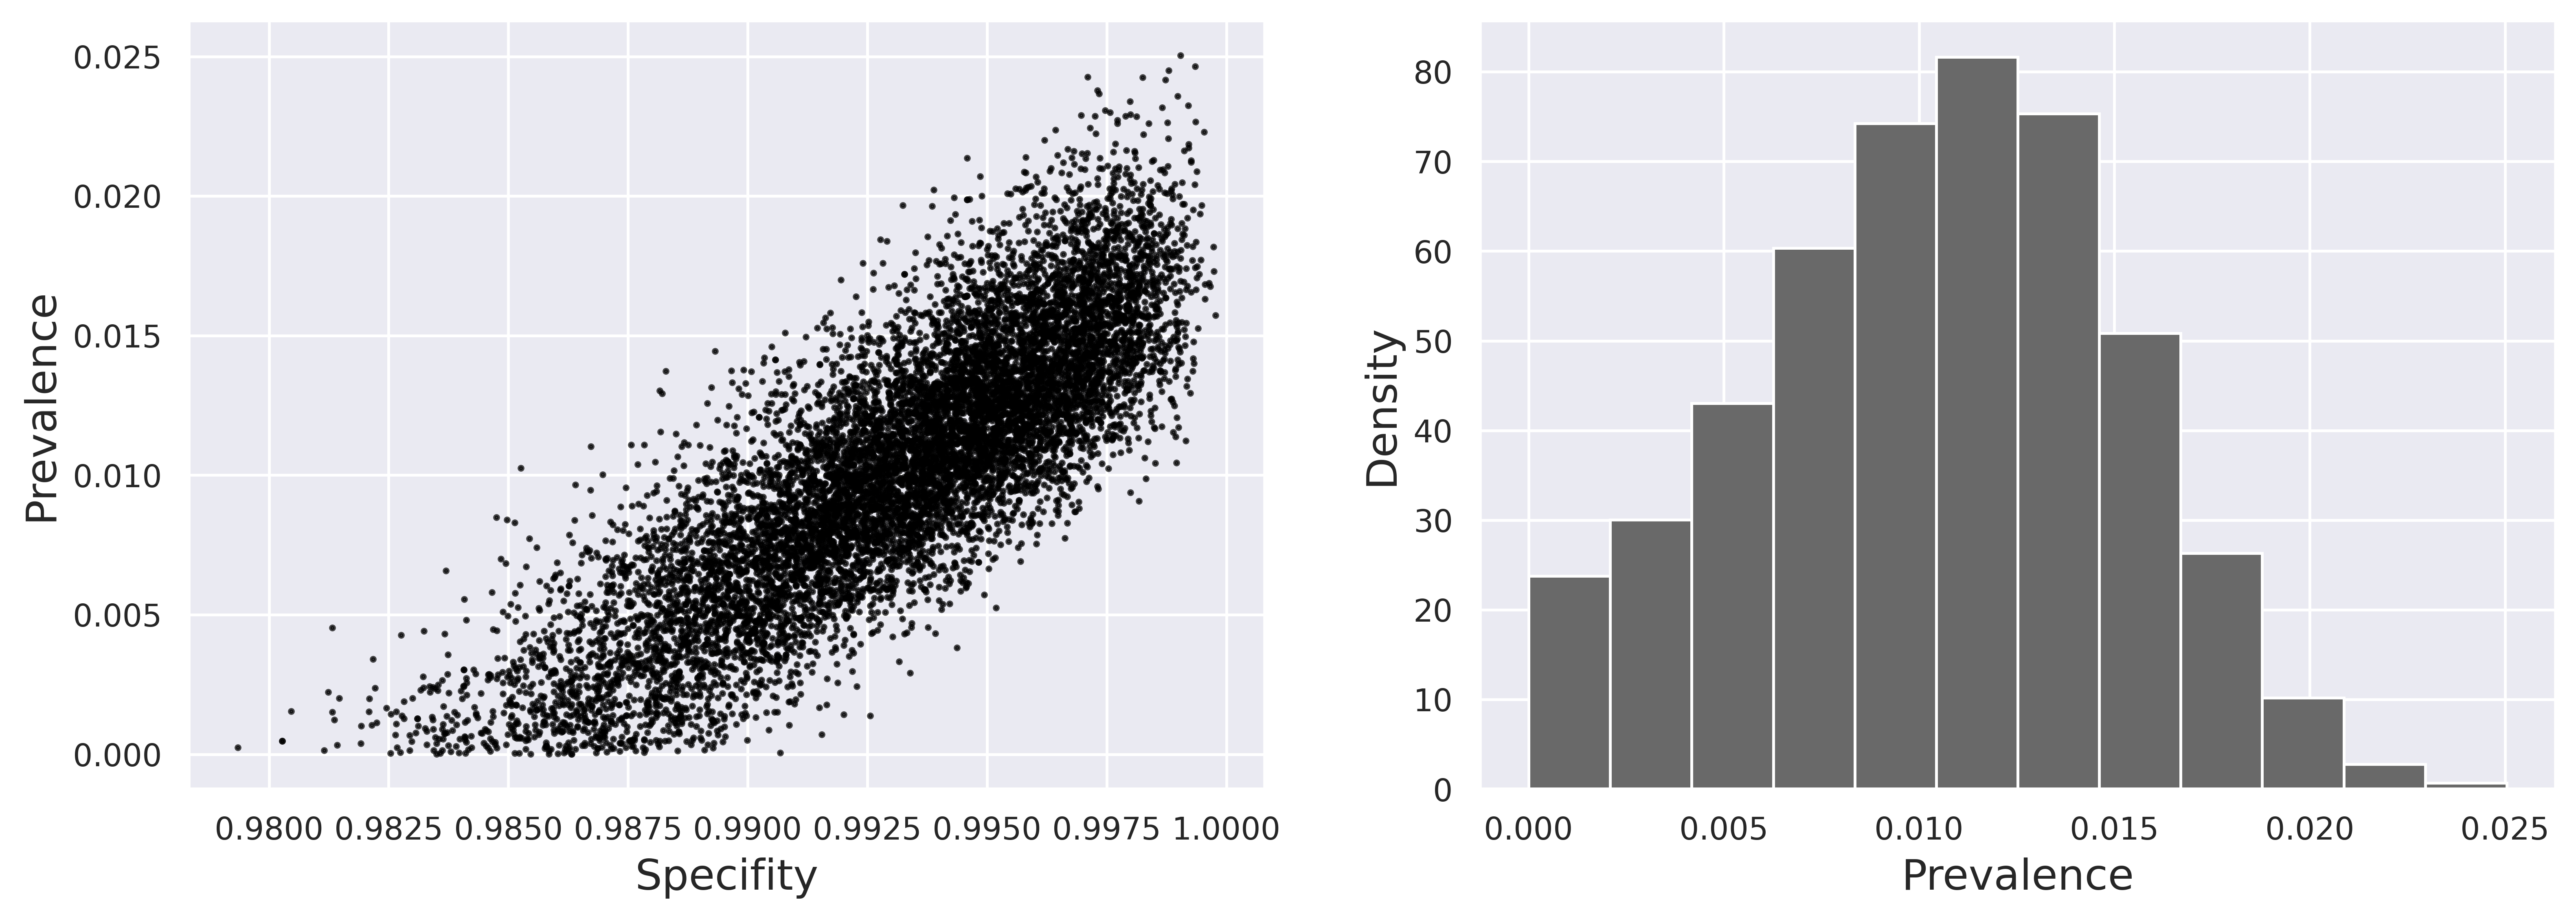
\includegraphics[width=\textwidth]{../../images/model1_gelman_figure_english.png}
  \caption{Scatter plot of posterior simulations of prevalence against
  specificity and histogram of posterior simulations of the prevalence.}
  \label{fig:results-posterior-model1}
\end{figure}

Other approach considers more than one study about specificity and
sensitivity. A {\em hierarchical partial pooling} model for these studies
can be done in the following way: 
\begin{gather*}
    \operatorname{logit}(\gamma_s^j) \sim \operatorname{Normal}(\mu_{\gamma_s}, \sigma_{\gamma_s}), \\
    \operatorname{logit}(\gamma_e^j) \sim \operatorname{Normal}(\mu_{\gamma_e}, \sigma_{\gamma_e}), 
\end{gather*}
for $1 \le j \le K$ studies, such that the first study is the considered one.
Partial pooling because the parameters can be sampled from the same
distribution. Hierarchical because the parameters of this distribution have
its one prior distributions. For instance, 
\begin{align*}
    \mu_{\gamma_s} &\sim N(0, 10), \\ 
    \mu_{\gamma_e} &\sim N(0, 10), \\
    \sigma_{\gamma_s} &\sim N^+(0,1), \text{ and } \\
    \sigma_{\gamma_e} &\sim N^+(0,1),
\end{align*}
where $N^+(a,b)$ is the truncated normal distribution in $[0,+\infty)$. All
the codes available at Github
repository\footnote{\url{https://github.com/lucasmoschen/rds-bayesian-analysis}}.

Finally, we studied a joint distribution for specificity and sensitivity, a
possible bivariate beta distribution built in \cite{olkin2015constructions}.
This distribution is derived from a Dirichlet distribution of order four. Let $U = (U[1],...,U[4]) \sim \operatorname{Dirichlet}(\boldsymbol{\alpha})$, where
$\boldsymbol{\alpha} \in \mathbb{R}^4_+$. Therefore, defining $X = U[1] +
U[2]$ and $Y = U[1] + U[3]$, we will have that $(X,Y)$ has a well-defined
probability distribution in
$[0,1] \times [0,1]$ such that $X$ and $Y$ have marginally beta distributions,
and they have correlation in all space. Depending on the definition of
$\boldsymbol{\alpha}$, the correlation between the variables range from -1 and
1. Figure \ref{fig:beta-bivariate} shows some examples of this construction. 

\begin{figure}[!ht]
    \centering
    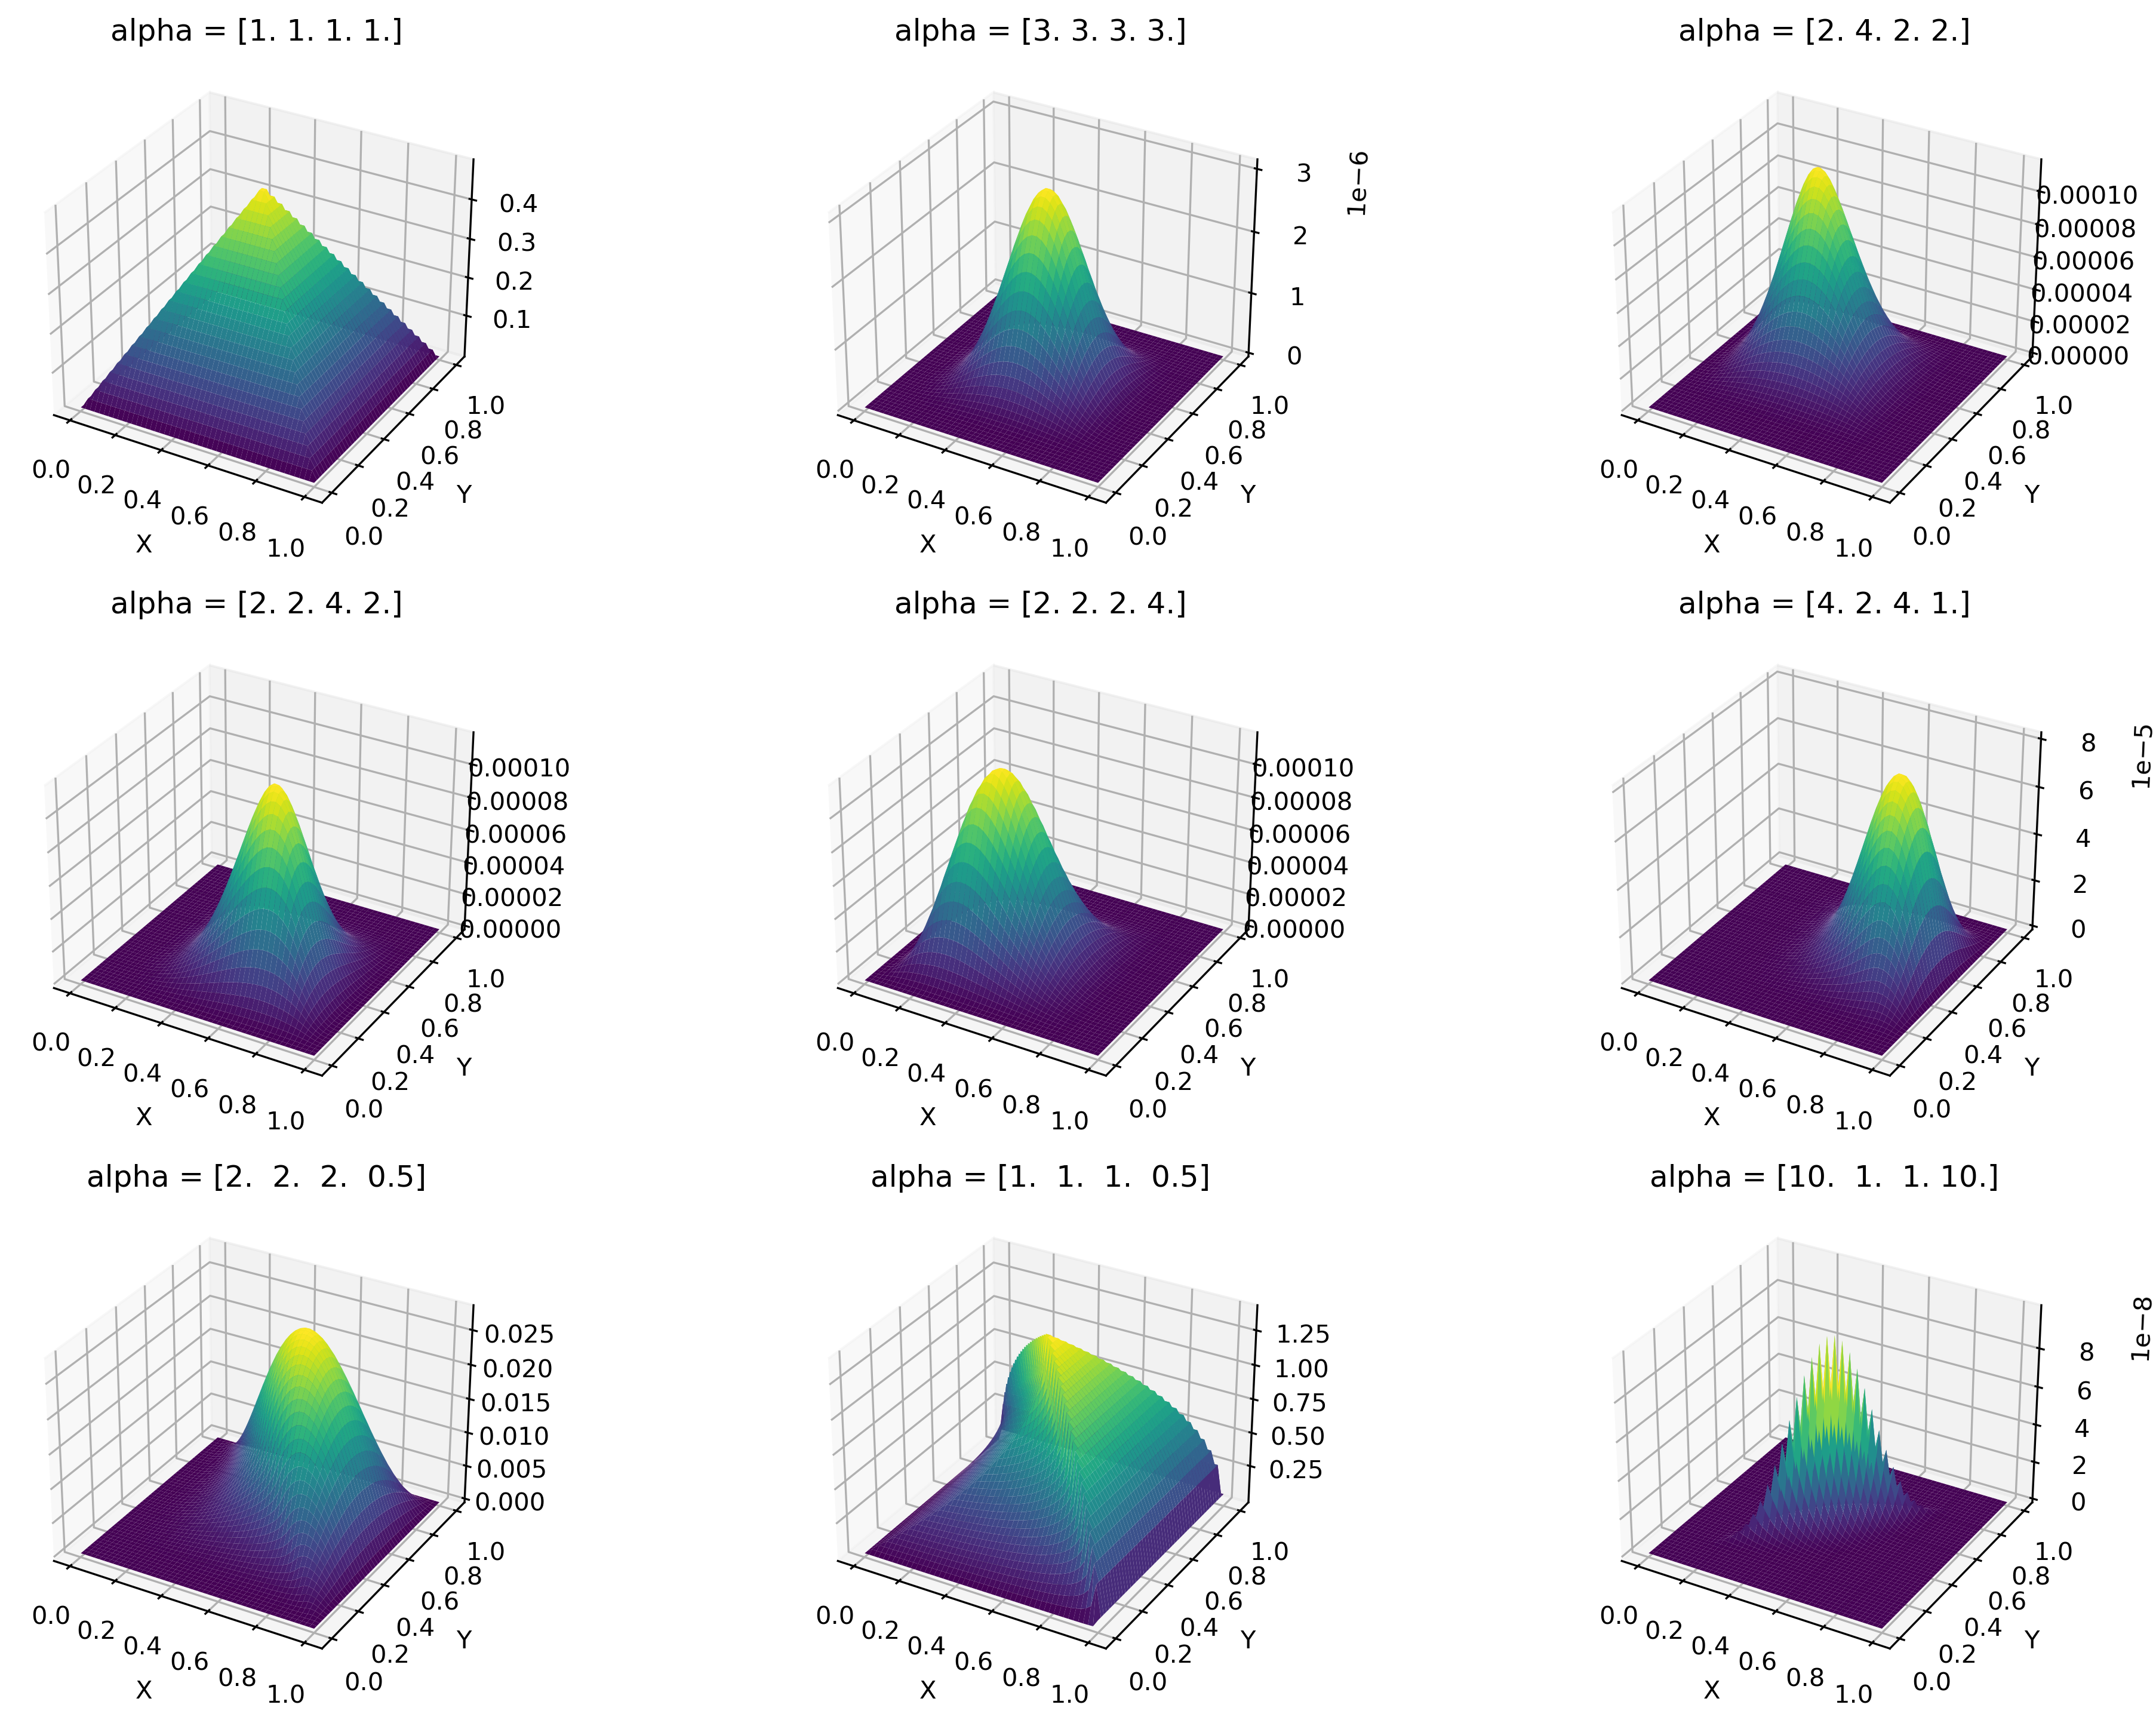
\includegraphics[width=\textwidth]{beta-distributions.png}
    \caption{Different choices of $\alpha$ and the joint distribution of the variables $X$ and $Y$.}
    \label{fig:beta-bivariate}
\end{figure}

\subsection{Imperfect tests and respondent-driven sampling}

For now, we consider the network dependence induced by the RDS with no
associated model. Therefore, we treat it as a random effect for
each individual. Conditionally autoregressive (CAR) models in the
Gaussian case are used. Let $[\tilde{Q}]_{ij} = \tilde{q}_{ij}$ be a fixed matrix which measures the distance between $i$
and $j$, and $\tilde{q}_{i+} = \sum_{j} \tilde{q}_{ij}$. In general, we use
$$
\tilde{q}_{ij} = \begin{cases}
  1, &\text{if } i \text{ recruited } j \text{ or the contrary} \\
  0, &\text{otherwise.} 
\end{cases}
$$
Next we define the scaled adjacency matrix $Q = D^{-1}\tilde{Q}$, such that $D$
is a diagonal matrix with $D_{ii} = \tilde{q}_{i+}$. Finally let $|\rho| < 1$ be a
parameter to controls the dependence between neighbors. Hence, we specify the
model as follows:

\begin{equation}
  \begin{aligned}
    T_i &\sim \bern(p_i) \\
    p_i &= \gamma_s\theta_i + (1-\gamma_e)(1 - \theta_i),  \\
    g(\theta_i) &= g(\theta) + \x_i^T\beta + \omega_i,  \\
    \omega_i|\{\omega_j\}_{j\neq i}, \tau &\sim \N\left(\rho\sum_j q_{ij}\omega_j, \tau^{-1}/\tilde{q}_{i+}\right) \\
    \beta &\sim \N(\mu, \Sigma), \\ 
    \theta &\sim \betadist(a^p, b^p) \\
    \gamma_s &\sim \betadist(a^s, b^s), \\
    \gamma_e &\sim \betadist(a^e, b^e), \\  
    \tau &\sim \operatorname{Gamma}(a^{\tau}, b^{\tau}).
  \end{aligned}  
\end{equation}
By Brook's Lemma \cite[]{brook1964distinction}, the joint distribution of
$\omega$ can be specified as 
$$
\omega \sim \N\left(0, \left[\tau (D - \rho \tilde{Q})\right]^{-1}\right).
$$

\subsubsection{Exponential Random Graph Model (ERGM)}

RDS has the constraint of being without replacement. For that reason, we do
not observe all links among the samples \cite[]{crawford2016}. Considering the
model developed by Crawford, we can model the
matrix $Q$ as {\em Exponential Random Graph Model} (ERGM). Define the
following 

\begin{enumerate}
  \item $\boldsymbol{s} = \tril(QC)^T \boldsymbol{1} + C^Tu$, such that $Q$ is the
  adjacency matrix of the recruited subjects, $C$ is the {\em Coupon Matrix},
  $u$ the vector of the number of edge ends belonging to each vertex
  (in the order of recruitment) that are not connected to any other sampled
  vertex, and $\tril(M)$ the lower triangle of $M$. 

  \item $T(Q) = -\lambda \boldsymbol{s}$, such that $\lambda$ is the rate of
  the recruitment time. 

  \item $V(Q) = \sum_{k \text{ is not seed}} \log(\lambda \boldsymbol{s}_k)$
  
  \item $w = (0, t_2 - t_1, ..., t_n - t_{n-1})$ is the vector of the waiting times between
  recruitments.  
\end{enumerate}

Therefore $\Pr(Q|w) \propto \exp[T(Q)^Tw + V(Q)]$. With that, the model
becomes 

\begin{equation}
  \begin{aligned}
    T_i &\sim \bern(p_i) \\
    p_i &= \gamma_s\theta_i + (1-\gamma_e)(1 - \theta_i),  \\
    g(\theta_i) &= g(\theta) + \x_i^T\beta + \omega_i,  \\
    \omega_i|\{\omega_j\}_{j\neq i}, \tau &\sim \N\left(\rho\sum_j q_{ij}\omega_j/q_{i+}, \tau^2/q_{i+}\right) \\
    Q|w &\propto \exp[T(Q)^Tw + V(Q)] \\
    \lambda &\sim \Gamma(a^{\lambda}, b^{\lambda}), \\ 
    \beta &\sim \N(\mu, \Sigma), \\ 
    \theta &\sim \betadist(a^p, b^p) \\
    \gamma_s &\sim \betadist(a^s, b^s), \\
    \gamma_e &\sim \betadist(a^e, b^e), \\  
    \tau &\sim \N^+(0,\sigma^2_{\tau}).
  \end{aligned}  
\end{equation}
The problem with this model is that we are assigning a posterior distribution
for $Q$.

\chapter{Respondent-driven sampling}

Respondent-driven sampling (RDS) is commonly used to survey hidden or hard-to-reach populations when
no sampling frame exists \cite[]{heckathorn1997}, which means there is no
enumeration of the population, since size and boundaries are unknown. In this approach, the
researchers select some individuals, called {\em seeds} from the target
population, and give them a fixed amount of {\em recruitment coupons} to
recruit their peers. Each recipient of the coupons reclaims it in the study
site, is interviewed, and receives more coupons to continue the recruitment.
This process occurs until some criteria is reached. The sampling is without
replacement, so the participants cannot be recruited more than once. Moreover,
the respondents inform how many subjects from the population they know.

The subjects receive a reward for being interviewed and for each recruitment
of their peers which establishes a dual incentive system. The {\em primary incentive} is the
{\em individual-sanction-based control}, so there is a reward for
participating. The second one is the {\em group-mediated social control} that
influences the participants to induce others to comply to get the reward for the recruitment. When social approval is important, recruitment can be even
more efficient and cheaper, since material incentive can be converted into
symbolic by the individuals. In summary, accepting to be recruited will have a
material incentive for both and a symbolic incentive for the recruited, since
theirs peers also participated.

Let $G = (V,E)$ be an undirected graph representing the hidden population. The {\em recruitment graph} $G_R =
(V_R, E_R)$ represents the recruited individuals and the recruitment edges,
that is, $(i,j) \in E_R$ if, and only if, $i$ recruited $j$.
Given that each individual can be sampled only once, it is not possible to
observe the {\em recruitment-induced subgraph}, that is the induced subgraph
generated by $V_R$. Moreover, the {\em coupon matrix} $C$ defined by $C_{ij} =
1$ if the i$^{th}$ subject has at least one coupon before the j$^{th}$
recruitment event, is also observed with the recruitment times. Assuming an
exponential and independent distribution of the times, the likelihood can be
written explicitly, and the distribution interpreted as an exponential random graph
model \cite[]{crawford2016}.  

These models allowed several applications in social sciences, epidemiology,
and statistics, including hidden populations size estimation
\cite[]{crawford2018hidden}, regression \cite[]{bastos2012binary}, communicable
disease prevalence estimation \cite[]{albuquerque2009avaliaccao}, among others.



\chapter{Specificity and sensitivity}

In this section, we shall describe how to use the Bivariate Beta
\cite[]{olkin2015constructions} to model the correlation between specificity
and sensitivity.

\section{Bivariate Beta construction}

Let $U = (U_1, U_2, U_3, U_4) \sim
\operatorname{Dirichlet}(\boldsymbol{\alpha})$, where $\boldsymbol{\alpha} =
(\alpha_1, \alpha_2, \alpha_3, \alpha_4)$ with $\alpha_i > 0, i = 1,\dots,4$
and $U_4 = 1 - U_1 + U_2 + U_3$. The joint density of $U$ with respect to the
Lebesgue measure is given by
\begin{equation}
  f_U(u_1, u_2, u_3) = \frac{1}{B(\boldsymbol{\alpha})}u_1^{\alpha_1-1}u_2^{\alpha_2-1}u_3^{\alpha_3-1}(1-u_1-u_2-u_3)^{\alpha_4-1}, 
\end{equation}
when $u_i \in [0,1], i = 1,2,3$, $u_1 + u_2 + u_3 \le 1$, and $0$ otherwise.
The normalizing constant is, for $v \in \R^n$,
$$B(v) = \frac{\prod_{i=1}^n \Gamma(v_i)}{\Gamma\left(\sum_{i=1}^n v_i\right)}.$$ 

\begin{definition}
  Let 
  \begin{equation}
    X = U_1 + U_2 \text{ and } Y = U_1 + U_3.
  \end{equation} 
    The distribution of $(X,Y)$ is {\em Bivariate Beta} with parameters
    $\boldsymbol{\alpha}$. 
\end{definition}

\begin{proposition}
  The marginal distribution of $X$ is Beta with parameters $\alpha_1 +
  \alpha_2$ and $\alpha_3 + \alpha_4$. Similarly, the marginal distribution of
  $Y$ is Beta with parameters $\alpha_1 + \alpha_3$ and $\alpha_2 + \alpha_4$.
\end{proposition}

\begin{proof}
  First we derive the probability density of $(U_1, U_2)$ with respect to the
  Lebesgue measure. 
  \begin{equation}
    \label{eq:dist-u1-u2}
    \begin{split}
      f_{U_1, U_2}(u_1, u_2) &= \int_{-\infty}^{\infty} f_{U}(u_1,u_2,u_3) \, du_3 \\ 
      &= \frac{1}{B(\boldsymbol{\alpha})}\int_0^1 u_1^{\alpha_1-1}u_2^{\alpha_2-1}u_3^{\alpha_3-1}(1-u_1-u_2-u_3)^{\alpha_4-1} \, du_3 \\
      &= \frac{1}{B(\boldsymbol{\alpha})}u_1^{\alpha_1-1}u_2^{\alpha_2-1}\int_0^1 u_3^{\alpha_3-1}(1-u_1-u_2-u_3)^{\alpha_4-1} \, du_3.
    \end{split}
  \end{equation}
  Let $u_3 = (1 - u_1 - u_2)z$. Then,
  \begin{equation}
    \begin{split}
      f_{U_1, U_2}(u_1, u_2) &= \frac{1}{B(\boldsymbol{\alpha})}u_1^{\alpha_1-1}u_2^{\alpha_2-1}\int_0^1 (1-u_1-u_2)^{\alpha_3-1}z^{\alpha_3-1}(1-u_1-u_2)^{\alpha_4}(1-z)^{\alpha_4-1} \, dz. \\
      &= \frac{1}{B(\boldsymbol{\alpha})}u_1^{\alpha_1-1}u_2^{\alpha_2-1}(1-u_1-u_2)^{\alpha_3+\alpha_4-1}\int_0^1 z^{\alpha_3-1}(1-z)^{\alpha_4-1} \, dz. \\
      &= \frac{1}{B(\boldsymbol{\alpha})}u_1^{\alpha_1-1}u_2^{\alpha_2-1}(1-u_1-u_2)^{\alpha_3+\alpha_4-1}\frac{\Gamma(\alpha_3)\Gamma(\alpha_4)}{\Gamma(\alpha_3 + \alpha_4)} \\
      &= \frac{1}{B(\alpha_1, \alpha_2, \alpha_3+\alpha_4)}u_1^{\alpha_1-1}u_2^{\alpha_2-1}(1-u_1-u_2)^{\alpha_3+\alpha_4-1}.
    \end{split}
  \end{equation}

We conclude that
$$(U_1, U_2, 1-U_1-U_2) \sim
\operatorname{Dirichlet}(\alpha_1,\alpha_2,\alpha_3+\alpha_4).$$

Define 
$$
H(v) = \begin{bmatrix}
  1 & 0 \\ 1 & 1
\end{bmatrix}v, \text{ for } v \in \R^2.
$$

Then $(U_1, X) = H(U_1, U_2)$ and $H(\cdot)$ is bijective and differentiable function. By the Change of Variable Formula, 
\begin{equation}
  \begin{split}
    f_{U_1, X}(u_1, x) &= f({H^{-1}(u_1,x)})\bigg|\det\left[\frac{dH^{-1}(v)}{dv}\bigg|_{v=(u_1,x)}\right]\bigg| \\ 
    &= f(u_1, x - u_1) = \frac{1}{B(\alpha_1, \alpha_2, \alpha_3+\alpha_4)}u_1^{\alpha_1-1}(x-u_1)^{\alpha_2-1}(1-x)^{\alpha_3+\alpha_4-1}, 
  \end{split}
\end{equation}
where $(u_1, x)$ belongs to the triangle defined by the points (0,0),
(0,1), and (1,1). The distribution of $X$ for $x \in [0,1]$ is
\begin{equation}
  \begin{split}
    f_X(x) &= \frac{1}{B(\alpha_1, \alpha_2, \alpha_3+\alpha_4)}\int_{0}^{x} u_1^{\alpha_1-1}(x-u_1)^{\alpha_2-1}(1-x)^{\alpha_3+\alpha_4-1} \, du_1 \\
    &= \frac{1}{B(\alpha_1, \alpha_2, \alpha_3+\alpha_4)}(1-x)^{\alpha_3+\alpha_4-1} \int_{0}^{x} u_1^{\alpha_1-1}(x-u_1)^{\alpha_2-1} \, du_1. \\
    &= \frac{1}{B(\alpha_1, \alpha_2, \alpha_3+\alpha_4)}(1-x)^{\alpha_3+\alpha_4-1} \int_{0}^{x} x^{\alpha_1-1} \left(\frac{u_1}{x}\right)^{\alpha_1-1}x^{\alpha_2 - 1}\left(1-\frac{u_1}{x}\right)^{\alpha_2-1} \, du_1. \\
  \end{split}
\end{equation}

Setting $u = u_1/x$ (if $x = 0, f_X(x) = 0$, then suppose $x > 0$), we have, 
\begin{equation}
  \begin{split}
    f_X(x) &= \frac{1}{B(\alpha_1, \alpha_2, \alpha_3+\alpha_4)}(1-x)^{\alpha_3+\alpha_4-1} x^{\alpha_1+\alpha_2-1} \int_{0}^{1} u^{\alpha_1-1}(1-u)^{\alpha_2-1} \, du. \\
    &= \frac{1}{B(\alpha_1, \alpha_2, \alpha_3+\alpha_4)}(1-x)^{\alpha_3+\alpha_4-1} x^{\alpha_1+\alpha_2-1} B(\alpha_1, \alpha_2)\\
    &= \frac{1}{B(\alpha_1 + \alpha_2, \alpha_3+\alpha_4)}(1-x)^{\alpha_3+\alpha_4-1} x^{\alpha_1+\alpha_2-1}\\
  \end{split}
\end{equation}
Therefore $X \sim \betadist(\alpha_1+\alpha_2, \alpha_3+\alpha_4)$. Similarly $Y \sim \betadist(\alpha_1+\alpha_3, \alpha_2 + \alpha_4)$.

\end{proof}

\begin{proposition}
  The joint density of $(X,Y)$ with respect to the Lebesgue measure is
  given by 
  \begin{equation}
    f_{X,Y}(x,y) = \frac{1}{B(\boldsymbol{\alpha})}\int_{\Omega} u_1^{\alpha_1 - 1}(x - u_1)^{\alpha_2 -1}(y-u_1)^{\alpha_3-1}(1-x-y+u_1)^{\alpha_4-1} \, du_1,
  \end{equation}
  where 
  $$
  \Omega = (\max(0, x+y-1), \min(x,y)).
  $$
\end{proposition}

\begin{proof}
  Note that
  $$
  \begin{bmatrix}
    U_1 \\ X \\ Y
  \end{bmatrix}  = \begin{bmatrix}
    1 & 0 & 0 \\
    1 & 1 & 0 \\
    1 & 0 & 1
  \end{bmatrix}\begin{bmatrix}
    U_1 \\ U_2 \\ U_3
  \end{bmatrix}, 
  $$
  where the linear function is bijective and differentiable function, such
  that the determinant of the derivative is 1. By the Change of Variable
  Formula, 
  \begin{equation}
    \begin{split}
      f_{U_1,X,Y}(u_1,x,y) &= f_{U_1,U_2,U_3}(u_1, x - u_1, y - u_2) \\ 
      &= \frac{1}{B(\boldsymbol{\alpha})}u_1^{\alpha_1-1}(x-u_1)^{\alpha_2-1}(y-u_1 )^{\alpha_3-1}(1-x-y+u_1)^{\alpha_4-1},
    \end{split}
  \end{equation}
  where $0 \le u_1 \le x, u_1 \le y$, and $0 \le 1 - x - y + u_1$.  
  Hence,
  \begin{equation}
      \label{eq:dist-X-Y}
      f_{X,Y}(x,y) = \frac{1}{B(\boldsymbol{\alpha})}\int_{\Omega} u_1^{\alpha_1-1}(x-u_1)^{\alpha_2-1}(y-u_1)^{\alpha_3-1}(1-x-y+u_1)^{\alpha_4-1} \, du_1,
  \end{equation}
  such that $\Omega = \{u_1 : \max(0, x + y -1) < u_1 < \min(x,y)\}$.
\end{proof}

\begin{proposition}
  The covariance between $X$ and $Y$ is 
  $$\cov(X,Y) = \frac{1}{\tilde{\alpha}^2(\tilde{\alpha}+1)}(\alpha_1\alpha_4 - \alpha_2\alpha_3).$$
\end{proposition}

\begin{proof}

  Let $\tilde{a} = \sum_i \alpha_i$. The covariance between $U_i$ and $U_j$ is \cite[]{lin2016dirichlet} 
\begin{equation}
  \cov(U_i, U_j) = - \frac{\alpha_i\alpha_j}{\tilde{\alpha}^2(\tilde{\alpha}+1)}, i,j = 1,...,4, i \neq j
\end{equation} 
and the variance of $U_i$ is 
\begin{equation}
  \var(U_i) = \frac{\alpha_i(\tilde{\alpha}-\alpha_i)}{\tilde{\alpha}^2(\tilde{\alpha}+1)},
\end{equation}
since $U_i \sim \operatorname{Beta}(\alpha_i, \tilde{\alpha} -\alpha_i)$.
Therefore 
\begin{equation}
  \cov(X,Y) = \cov(U_1+U_2, U_1+U_3) = \frac{1}{\tilde{\alpha}^2(\tilde{\alpha}+1)}(\alpha_1\alpha_4 - \alpha_2\alpha_3)
\end{equation}
  
\end{proof}

The main moments of $X$ and $Y$ are the following 
\begin{align*}
    \ev(X) &= \ev(U_1 + U_2) = \frac{\alpha_1+\alpha_2}{\alpha_1+\alpha_2+\alpha_3+\alpha_4} \\
    \ev(Y) &= \ev(U_1 + U_3) = \frac{\alpha_1+\alpha_3}{\alpha_1+\alpha_2+\alpha_3+\alpha_4} \\
    \var(X) &= \cov(U_1+U_2, U_1+U_2) = \frac{1}{\tilde{\alpha}^2(\tilde{\alpha}+1)}(\alpha_1+\alpha_2)(\alpha_3 + \alpha_4) \\
    \var(Y) &= \cov(U_1+U_3, U_1+U_3) = \frac{1}{\tilde{\alpha}^2(\tilde{\alpha}+1)}(\alpha_1+\alpha_3)(\alpha_2 + \alpha_4)  \\  
    \cor(X,Y) &= \frac{\cov(X,Y)}{\sqrt{\var(X)\var(Y)}} = \frac{\alpha_1\alpha_4 - \alpha_2\alpha_3}{\sqrt{(\alpha_1+\alpha_2)(\alpha_3+\alpha_4)(\alpha_1+\alpha_3)(\alpha_2+\alpha_4)}}
\end{align*}

The original paper has a mistake in page
6\footnote{\url{https://www.wolframalpha.com/input/?i=simplify+\%28a\%28a\%2B1\%29+\%2B+a*b+\%2B+a*c+\%2B+b*c\%29\%2F\%28\%28a\%2Bb\%2Bc\%2Bd\%29*\%28a\%2Bb\%2Bc\%2Bd\%2B1\%29\%29+-+\%28a+\%2B+b\%29*\%28a\%2Bc\%29\%2F\%28a\%2Bb\%2Bc\%2Bd\%29\%5E2+}}.

\section{Comments about integration}

The density of $(X,Y)$ with respect to the Lebesgue measure is $f_{X,Y}(x,y)$
as in equation \eqref{eq:dist-X-Y}. Therefore it can be undefined in sets of
null Lebesgue measure in $\R^2$. This section
aims to find them to help writing the function properly. If $\alpha_i \ge 1,
\, i = 1,...,4$, the integral is clearly well defined for every $x,y \in [0,1]$. Let $0 < \alpha_2 = \alpha_3 = a \le 0.5$ and $x = y < 0.5$. Then
\begin{equation*}
  \begin{split}
    f_{X,Y}(x,y) &= \frac{1}{B(\boldsymbol{\alpha})}\int_{0}^x u_1^{\alpha_1-1}(x-u_1)^{a-1}(x-u_1)^{a-1}(1-2x+u_1)^{\alpha_4-1} \, du_1 \\
    &= \frac{1}{B(\boldsymbol{\alpha})}\int_{0}^{x/2} u_1^{\alpha_1-1}(x-u_1)^{2a-2}(1-2x+u_1)^{\alpha_4-1} \, du_1 + \\
    &~~~+ \frac{1}{B(\boldsymbol{\alpha})}\int_{x/2}^x u_1^{\alpha_1-1}(x-u_1)^{2a-2}(1-2x+u_1)^{\alpha_4-1} \, du_1
  \end{split}
\end{equation*}

Note that the first integral is well defined and non-negative. If $\alpha_1 \ge 1$, 
\begin{equation*}
  \begin{split}
    \int_{0}^{x/2} u_1^{\alpha_1-1}&(x-u_1)^{2a-2}(1-2x+u_1)^{\alpha_4-1} \, du_1 \\
    &\le \int_{0}^{x/2} \frac{x}{2}^{\alpha_1-1}\left(\frac{x}{2}\right)^{2a-2}\max\left(\left(1-\frac{3}{2}x\right)^{\alpha_4-1}, (1-2x)^{\alpha_4-1}\right) \, du_1 < +\infty.
  \end{split}
\end{equation*}

If $0 < \alpha_1 < 1$, 
\begin{equation*}
  \begin{split}
    \int_{0}^{x/2} u_1^{\alpha_1-1}&(x-u_1)^{2a-2}(1-2x+u_1)^{\alpha_4-1} \, du_1 \\
    &= \lim_{t\to 0^+}\int_{t}^{x/2} u_1^{\alpha_1-1}\left(\frac{x}{2}\right)^{2a-2}\max\left(\left(1-\frac{3}{2}x\right)^{\alpha_4-1}, (1-2x)^{\alpha_4-1}\right) \, du_1 \\ 
    &= K(x)\lim_{t\to 0^+}\int_{t}^{x/2} u_1^{\alpha_1-1}\, du_1 \\ 
    &= \frac{K(x)}{\alpha_1}\lim_{t\to 0^+} \, \left[\left(\frac{x}{2}\right)^{\alpha_1} - t^{\alpha_1}\right] < +\infty .\\ 
  \end{split}
\end{equation*}
where $K(x)$ is a function of $x$. Moreover, since the integrand is non-negative, so is the integral. On the
other hand, the second integral is not defined: 
\begin{equation*}
  \begin{split}
    \int_{x/2}^{x} u_1^{\alpha_1-1}&(x-u_1)^{2a-2}(1-2x+u_1)^{\alpha_4-1} \, du_1 \\
    &\ge \int_{x/2}^x \min\left(\left(\frac{x}{2}\right)^{\alpha_1-1}, x^{\alpha_1-1}\right)(x-u_1)^{2a-2}\min\left(\left(1-\frac{3}{2}x\right)^{\alpha_4-1}, (1-x)^{\alpha_4-1}\right) \, du_1 \\
    &= K'(x) \int_{0}^{x/2} v^{2a-2} \, dv \\ 
    &= \begin{cases}
      \dfrac{K'(x)}{2a-1} \lim_{t \to 0^+} \left[(x/2)^{2a-1} - t^{2a-1}\right] &\text{ if } a < 0.5 \\ 
      K'(x) \lim_{t \to 0^+} \left[\log(x/2) - \log(t)\right] &\text{ if } a = 0.5
    \end{cases} \\
    &\to +\infty.
  \end{split}
\end{equation*}

Based on this divergence, we conclude that if $0 < \alpha_2 = \alpha_3 \le 0.5$
and $x = y < 0.5$, $f_{X,Y}(x,y)$ is not defined. Note that if $x = y \ge
0.5$, divergence problems still happens, since the problems appear when $u_1$
converges to $x$. Similar calculations show
that if $x + y = 1$ and $0 < \alpha_1 = \alpha_4 \le 0.5$, the density is also
not defined. More generally, $f_{X,Y}(x,y)$ is not defined if 

\begin{enumerate}
  \item $\alpha_1 + \alpha_4 \le 1$ and $x + y = 1$. 
  \item $\alpha_2 + \alpha_3 \le 1$ and $x = y$. 
\end{enumerate}

\section{Specifying parameters
\texorpdfstring{$\boldsymbol{\alpha}$}{alpha}}

Suppose that the researcher has knowledge about the main moments of $X$ and
$Y$, such that $\ev(X) = m_1 \in (0,1), \ev(Y) = m_2 \in (0,1), \var(X) = v_1
\in (0, 1),$ and $\var(Y) =
v_2 \in (0,1)$. Notice that $v_1 + m_1^2 = \var(X_1) + \ev[X_1]^2 = \ev[X_1^2]$ and
$$
\ev[X_1^2] - \ev[X_1] = \frac{(\alpha_1 + \alpha_2 + 1)(\alpha_1 + \alpha_2)}{(\tilde{\alpha} + 1)\tilde{\alpha}} - \frac{\alpha_1 + \alpha_2}{\tilde{\alpha}} = -\frac{(\alpha_1 + \alpha_2)(\alpha_3 + \alpha_4)}{\tilde{\alpha}(\tilde{\alpha}+1)} < 0, 
$$
that is, $v_1 + m_1^2 - m_1 < 0 \implies v_1 < m_1 - m_1^2$ and similarly,
$v_2 < m_2 - m_2^2$. After fixing these quantities, we will have a non-linear system with four equations and four
unknown variables. Hence, we want to solve the following 
\begin{equation}
  \label{eq:system-moments-alpha}
  \begin{cases}
    m_1 = \dfrac{\alpha_1+\alpha_2}{\tilde{\alpha}} \\
    m_2 = \dfrac{\alpha_1+\alpha_3}{\tilde{\alpha}} \\ 
    v_1 = \dfrac{(\alpha_1+\alpha_2)(\alpha_3+\alpha_4)}{\tilde{\alpha}^2(\tilde{\alpha}+1)} = m_1\dfrac{\alpha_3+\alpha_4}{\tilde{\alpha}(\tilde{\alpha}+1)} \\
    v_2 = \dfrac{(\alpha_1+\alpha_3)(\alpha_2+\alpha_4)}{\tilde{\alpha}^2(\tilde{\alpha}+1)} = m_2\dfrac{\alpha_2+\alpha_4}{\tilde{\alpha}(\tilde{\alpha}+1)}.
  \end{cases}
\end{equation}

\begin{proposition}
  System \eqref{eq:system-moments-alpha} has a solution if, and only if, the relation
  \begin{equation}
    \label{eq:v2}
    v_2 = \frac{(1 - m_2)\tilde{\alpha}}{\tilde{\alpha}(\tilde{\alpha}+ 1)} = \frac{1 - m_2}{\frac{m_1 - m_1^2}{v_1}} = \frac{v_1(1 - m_2)}{m_1(1-m_1)},
  \end{equation}
  is satisfied. When there is a solution, there will be
  infinitely many and they all lay in the ray 
  $$
\mathcal{L} = \{(1,-1,-1,1)\alpha_4 + k : \alpha_4 > 0\}, 
$$
such that $k = \left((m_1 + m_2 - 1)\tilde{\alpha}, (1-m_2)\tilde{\alpha},
(1-m_1)\tilde{\alpha}, 0\right)$. 
\end{proposition}

\begin{proof}
  

The first two equations of the system \eqref{eq:system-moments-alpha} can be
rewritten as a linear system:
\begin{align*}
  (m_1 - 1)\alpha_1 + (m_1 - 1)\alpha_2 + m_1\alpha_3 + m_1\alpha_4 &= 0 \\
  (m_2 - 1)\alpha_1 + m_2\alpha_2 + (m_2-1)\alpha_3 + m_2\alpha_4 &= 0,   
\end{align*}
which is equivalent to 
\begin{align*}
  \alpha_1 + \alpha_2 + \frac{m_1}{m_1-1}\alpha_3 + \frac{m_1}{m_1-1}\alpha_4 &= 0 \\
  \alpha_2 + \frac{1-m_2}{m_1-1}\alpha_3 + \frac{m_1-m_2}{m_1-1}\alpha_4 &= 0.
\end{align*}
Then, we can write $\alpha_1$ and $\alpha_2$ as functions of $\alpha_3$ and
$\alpha_4$:
\begin{align}
  \alpha_1 &= \frac{m_1+m_2-1}{1-m_1}\alpha_3 + \frac{m_2}{1-m_1}\alpha_4 \\
  \alpha_2 &= \frac{1-m_2}{1-m_1}\alpha_3 + \frac{m_1-m_2}{1-m_1}\alpha_4.
\end{align}
With that expression, let $\alpha_1 = a_3\alpha_3 + a_4\alpha_4$ and $\alpha_2
= b_3\alpha_3 + b_4\alpha_4$. Denote $c_3 = a_3 + b_3 + 1$ and $c_4 = a_4 +
b_4 + 1$. Then, consider the third equation of the system
\eqref{eq:system-moments-alpha}, 
\begin{equation*}
  \begin{split}
    &\frac{v_1}{m_1} = \frac{\alpha_3+\alpha_4}{\tilde{\alpha}(\tilde{\alpha} +1)} = \frac{\alpha_3+\alpha_4}{(\alpha_1+\alpha_2+\alpha_3+\alpha_4)^2 + (\alpha_1+\alpha_2+\alpha_3+\alpha_4)} \\
     &\implies \frac{v_1}{m_1}(\alpha_1 + \alpha_2 + \alpha_3 + \alpha_4)^2 = \alpha_3 + \alpha_4 - \frac{v_1}{m_1}(\alpha_1 + \alpha_2 + \alpha_3 + \alpha_4) \\
    &\implies \frac{v_1}{m_1}(c_3\alpha_3 + c_4\alpha_4)^2 = \left(1-\frac{v_1}{m_1}c_3\right)\alpha_3 + \left(1-\frac{v_1}{m_1}c_4\right)\alpha_4 \\
    &\implies \frac{v_1c_3^2}{m_1}\alpha_3^2 + \left(\frac{2v_1c_3c_4\alpha_4+v_1c_3}{m_1} - 1\right)\alpha_3 + \left(\frac{v_1c_4^2\alpha_4^2 + v_1c_4\alpha_4}{m_1} - \alpha_4\right) = 0 \\ 
    &\implies v_1c_3^2\alpha_3^2 + (2v_1c_3c_4\alpha_4+v_1c_3 - m_1)\alpha_3 + (v_1c_4^2\alpha_4^2 + v_1c_4\alpha_4 - m_1\alpha_4) = 0.
  \end{split}
\end{equation*}
Using a Computer Algebra System (CAS) with the Python library SymPy, the above
expression can be simplified as follows:
$$
v_1\alpha_3^2 + \left(v_1(1-m_1) + 2v_1\alpha_4 - m_1(1-m_1)^2\right)\alpha_3 - \alpha_4m_1(1-m_1)^2 + \alpha_4v_1(1 - m_1) + v_1\alpha_4^2 = 0.
$$
This way, the solutions of the above equation are function of $\alpha_4$.
Therefore, after solving the equations, we can use the last equation of the
system \eqref{eq:system-moments-alpha} as a function on of $\alpha_4$. Let, 
$$
\Lambda = \left(v_1(1-m_1) + v_1\alpha_4 - m_1(1-m_1)^2\right).
$$
Then, 
\begin{equation*}
  \begin{split}
    \Delta &= \left(v_1(1-m_1) + 2v_1\alpha_4 - m_1(1-m_1)^2\right)^2 - 4v_1(\alpha_4v_1(1 - m_1) - \alpha_4m_1(1-m_1)^2 + v_1\alpha_4^2), \\
    &= \left(\Lambda + v_1\alpha_4\right)^2 - 4v_1\alpha_4\Lambda \\
    &= \Lambda^2 - 2\Lambda v_1\alpha_4 + (v_1\alpha_4)^2 \\
    &= (\Lambda - v_1\alpha_4)^2 \\
    &= \left(v_1(1-m_1) - m_1(1-m_1)^2\right)^2 \\ 
    &= (1 - m_1)^2(v_1 + m_1^2 - m_1)^2.
  \end{split}
\end{equation*}
Note that $v_1 + m_1^2 = \var(X_1) + \ev[X_1]^2 = \ev[X_1^2]$ and
$$
\ev[X_1^2] - \ev[X_1] = \frac{(\alpha_1 + \alpha_2 + 1)(\alpha_1 + \alpha_2)}{(\tilde{\alpha} + 1)\tilde{\alpha}} - \frac{\alpha_1 + \alpha_2}{\tilde{\alpha}} = -\frac{(\alpha_1 + \alpha_2)(\alpha_3 + \alpha_4)}{\tilde{\alpha}(\tilde{\alpha}+1)} < 0.
$$
Therefore, 
$$
\sqrt{\Delta} = (1-m_1)(m_1 - v_1 - m_1^2)
$$
and 
\begin{equation*}
  \begin{split}
    \alpha_3 &= \frac{1}{2v_1}\left(\left(m_1(1-m_1)^2 - v_1(1-m_1) - 2v_1\alpha_4\right) \pm (1-m_1)(m_1 - v_1 - m_1^2)\right) \\
    &= - \alpha_4 + \frac{(1-m_1)(m_1 - m_1^2 - v_1) \pm (1-m_1)(m_1-v_1-m_1^2)}{2v_1}.
  \end{split}
\end{equation*}
When the sign is negative, we have that $\alpha_3 = - \alpha_4$, an impossible
solution. Then, 
$$
\alpha_3 = \frac{(1-m_1)(m_1 - m_1^2 - v_1)}{v_1} - \alpha_4.
$$

We summarize the expressions in function of $\alpha_4$: 
\begin{align*}
  \alpha_3 &= \frac{(1-m_1)(m_1 - m_1^2 - v_1)}{v_1} - \alpha_4 \\
  \alpha_1 &= \frac{m_1+m_2-1}{1-m_1}\alpha_3 + \frac{m_2}{1-m_1}\alpha_4 = \frac{(m_1 + m_2 - 1)(m_1 - m_1^2 - v_1)}{v_1} + \alpha_4 \\
  \alpha_2 &= \frac{1-m_2}{1-m_1}\alpha_3 + \frac{m_1-m_2}{1-m_1}\alpha_4 = \frac{(1 - m_2)(m_1 - m_1^2 - v_1)}{v_1} - \alpha_4 .
\end{align*}

From here, one can calculate that
$$
\tilde{\alpha} = \frac{m_1 - m_1^2 - v_1}{v_1}.
$$
Since $\alpha_2 + \alpha_4 = (1 - m_2)\tilde{\alpha}$, we have that the last
equation of the system \eqref{eq:system-moments-alpha} is given by
\eqref{eq:v2}, that is, the system $\eqref{eq:system-moments-alpha}$ has a solution if and
only if, equation \eqref{eq:v2} is satisfied. If it is, the solution is the ray 
$$
\mathcal{L} = \{(1,-1,-1,1)\alpha_4 + k : \alpha_4 > 0\}, 
$$
such that $k = \left((m_1 + m_2 - 1)\tilde{\alpha}, (1-m_2)\tilde{\alpha},
(1-m_1)\tilde{\alpha}, 0\right)$. 

\end{proof}


Now change the fourth equation of \eqref{eq:system-moments-alpha} by: 
$$
\cor(X,Y) = \frac{\alpha_1\alpha_4 - \alpha_2\alpha_3}{\sqrt{(\alpha_1+\alpha_2)(\alpha_3+\alpha_4)(\alpha_1+\alpha_3)(\alpha_2+\alpha_4)}} = \frac{\alpha_1\alpha_4 - \alpha_2\alpha_3}{\tilde{\alpha}^2\sqrt{m_1m_2(1-m_1)(1-m_2)}}
$$

Supposing the expression for $\alpha_1, \alpha_2$ and $\alpha_3$, that is,
$m_1, m_2$ and $v_1$ are fixed, and supposing we fix $\rho = \cor(X,Y)$, we
can simplify the above expression (using a software) as follows: 

$$
\rho = \frac{1}{\tilde{\alpha}\sqrt{m_1m_2(1-m_1)(1-m_2)}}\alpha_4 - \sqrt{\frac{(1 - m_1)(1 - m_2)}{m_1m_2}},
$$
which is linear on $\alpha_4$, that is, for fixed values of
$m_1, m_2, v_1$ and $\rho$, there is an unique $\alpha_4$, and hence,
$\alpha_1, \alpha_2$ and $\alpha_3$ that satisfies system
\eqref{eq:system-moments-alpha} with the fourth equation changed by the
correlation. 

\chapter{Bayesian statistics}

There are two more common interpretations of probability and statistics:
frequentist and Bayesian. While the frequentists define
probability as the limit of a frequency in a large number of trials, the
Bayesians represent an individual's degree of belief in a statement that is
updated given new information. This philosophy allows assigning probabilities
to any event, even if a random process is not defined \cite{statisticat2016laplacesdemon}. 

In 1761, Reverend Thomas Bayes wrote for the first time the Bayes' formula
relating the probability of a parameter after observing the data with the
evidence (written through a likelihood function) and previous information
about the parameter. Pierre Simon Laplace rediscovered this formula in 1773
\cite{Robert2007}, and this theory became more common in the 19th century.
After some criticisms, a modern treatment considering Kolmogorov's axiomatization of the theory of probabilities started after Jeffreys in 1939.
The recent development of new computational tools brought these ideas again.

Bayesian inference is composed by the following: 

\begin{itemize}
    \item A distribution for the parameters $\theta$ that quantifies the
    uncertainty about $\theta$ before data;
    \item A distribution of the data generation process given the parameter,
    such that, when it is seen as function of the parameter, is called
    likelihood function;
    \item When considering decision theory, a loss function measuring the
    error in evaluating the parameter;
    \item Posterior distribution of the parameter conditioned on the data. All
    inferences are based on this probability distribution.
\end{itemize} 

A key quantity for epidemiologists and public health researchers is the
proportion of individuals exposed to a disease at time $t$, which is called
{\em prevalence}. When measured
periodically, its evolution can identify potential causes of the infection
and prevention and care methods \cite[]{noordzij2010measures}. The prevalence
differs from {\em incidence } that measures the proportion of people who
develop new disease during a specified period of time
\cite[]{rothman2008modern}. Therefore, prevalence reflects both incidence and the
duration of disease. 

This report presents the initial models for my bachelor dissertation entitled ``Bayesian analysis of respondent-driven surveys with
outcome uncertainty'', which proposes to study prevalence when the diagnostic
tests are imperfect and the population is hidden, that is, there is no
sampling frame for it \cite[]{heckathorn1997}. 


\begin{alineas}
    \item Descrição do problema em termos matemáticos e revisão bibliográfica:
    material sobre RDS (formalização matemática em forma de cadeia ou processo
    de ramificação), regressão logística em que a resposta tem incerteza e
    aplicações em usuários de drogas, infecções transmissíveis, entre outros. 
    \item Incerteza sobre especificidade e sensitividade do teste e como
    propagar a classificação errada na rede. Comparação de prioris e, por isso, estudo de
    métodos Bayesianos. Justificar utilização desses métodos com argumento da
    incerteza. 
    \item Estudo do MCMC e Aproximação de Laplace, comparação dos algoritmos
    em alguns artigos e, quem sabe, codificação em Python e R. 
    \item Implementação de inferência eficiente em INLA, com possibilidades
    abertas em Python (talvez Julia?)
\end{alineas}


\chapter{Conclusion}

Respondent-driven sampling is a useful tool when the population can not be
enumerated since by building a dual incentive system, it encourages the
individuals from the target population to engage in the research and convince
others to do the same. Analysis of RDS started with \textcite{heckathorn1997}
and much work has being done as a wall of bricks. The resulting structure of
the process needs many assumptions that need to be considered in our analysis.
This work proposed a method to quantity the uncertainty about the
characteristics of these populations, which is vital for correction of
expectations. 

Regression analysis is powerful toolbox of statistical procedures that help
the understanding of the populations, but ``with great power comes great
responsibility'' \cite[p. 13]{spider_man}. When correct analysis are not done,
problems of estimation, such as identifiability and biases, can lead to wrong
inferences. In this work, we showed the importance of identifiability and
possible solutions in the Bayesian paradigm. CAR models showed to be a good
representation of spatial correlation, but with hidden problems. The parameter of
correlation is very difficult to interpret and even high values can not
generate the correct expected spatial dependencies. However, these models
complicate the sampling by increasing the parameter space dimension. For an unbiased estimation of prevalence, this work presented the relevant 
role of sensitivity and specificity, in special when there considering theirs
uncertainties. 

We also analysed different prior specifications of sensitivity and specificity
since strong priors are required. We highlighted each one's advantages and
disadvantages. In particular, we detailed several characteristics of the
bivariate beta distribution derived by \textcite{olkin2015constructions}. This
distribution showed to have some specification problems since not all
information can be directly converted to a well-defined distribution. 

Other key aspect of Bayesian inference is the prior specification. It can save
our life in identification problems, but it can derive wrong results when
badly specified. In particular, when there is not much spatial correlation, a 
finite mean prior specification leads to divergences in the sampling method
and incorrect inferences. Prior information is not always easily converted to
prior distributions as we studied in the logit normal case. Prior and
posterior predictive checks are possible ways to understand the process. 

Analysis of HMC results and its diagnostics are very important for the
learning process. Observing divergences, mixing of the chain, energy of the
model, among other diagnoses can enlighten problems with the parametrization
of the model and indicate possible solution paths. 

Finally, the simulations indicated two important characteristics of the
presented model: the computational burden is high with a very complicated
geometry, and the inferences are consistent when HMC is well diagnosed and
prior specification is well thought.  

% -----------------------------------
% ELEMENTOS PÓS-TEXTUAIS
% -----------------------------------
\postextual
% ----------------------------------

%\bibliography{biblio}
\printbibliography

%\glossary

% ----------------------------------------------------------
% Apêndices
% ----------------------------------------------------------

\begin{apendicesenv}

\partapendices

\chapter{A bivariate beta distribution}
\label{appendix:bivariate-beta-distribution}

\textcite{olkin2015constructions} describe a bivariate distribution with beta
marginal distributions, positive probability over the space $[0,1] \times
[0,1]$, and correlations over the full range $(-1,1)$. In this section, we
derive it and analyse some of its consequences as prior distribution. 

\section{Construction of the distribution}

Let $U = (U_1, U_2, U_3, U_4) \sim
\operatorname{Dirichlet}(\boldsymbol{\alpha})$, where $\boldsymbol{\alpha} =
(\alpha_1, \alpha_2, \alpha_3, \alpha_4)$ with $\alpha_i > 0, i = 1,\dots,4$
and $U_4 = 1 - U_1 + U_2 + U_3$. The joint density of $U$ with respect to the
Lebesgue measure is given by
\begin{equation}
  f_U(u_1, u_2, u_3) = \frac{1}{B(\boldsymbol{\alpha})}u_1^{\alpha_1-1}u_2^{\alpha_2-1}u_3^{\alpha_3-1}(1-u_1-u_2-u_3)^{\alpha_4-1}, 
\end{equation}
when $u_i \in [0,1], i = 1,2,3$, $u_1 + u_2 + u_3 \le 1$, and $0$ otherwise.
The normalizing constant is defined for $v \in \R^n$ as
$$B(v) = \frac{\prod_{i=1}^n \Gamma(v_i)}{\Gamma\left(\sum_{i=1}^n v_i\right)}.$$ 
\begin{definition}
  Let 
  \begin{equation}
    X = U_1 + U_2 \text{ and } Y = U_1 + U_3.
  \end{equation} 
    The distribution of $(X,Y)$ is {\em bivariate beta} with parameter
    $\boldsymbol{\alpha}$. 
\end{definition}

\autoref{fig:beta-bivariate} presents the joint density of $X$ and $Y$ for
different values of $\boldsymbol{\alpha}$. The following two propositions describe the marginal and joint
densities of
bivariate beta distribution. Their proofs are in the Appendix. 

\begin{figure}[!ht]
  \centering
  \caption{Joint density of the variables $X$ and $Y$ for different choices of $\boldsymbol{\alpha}$.}
  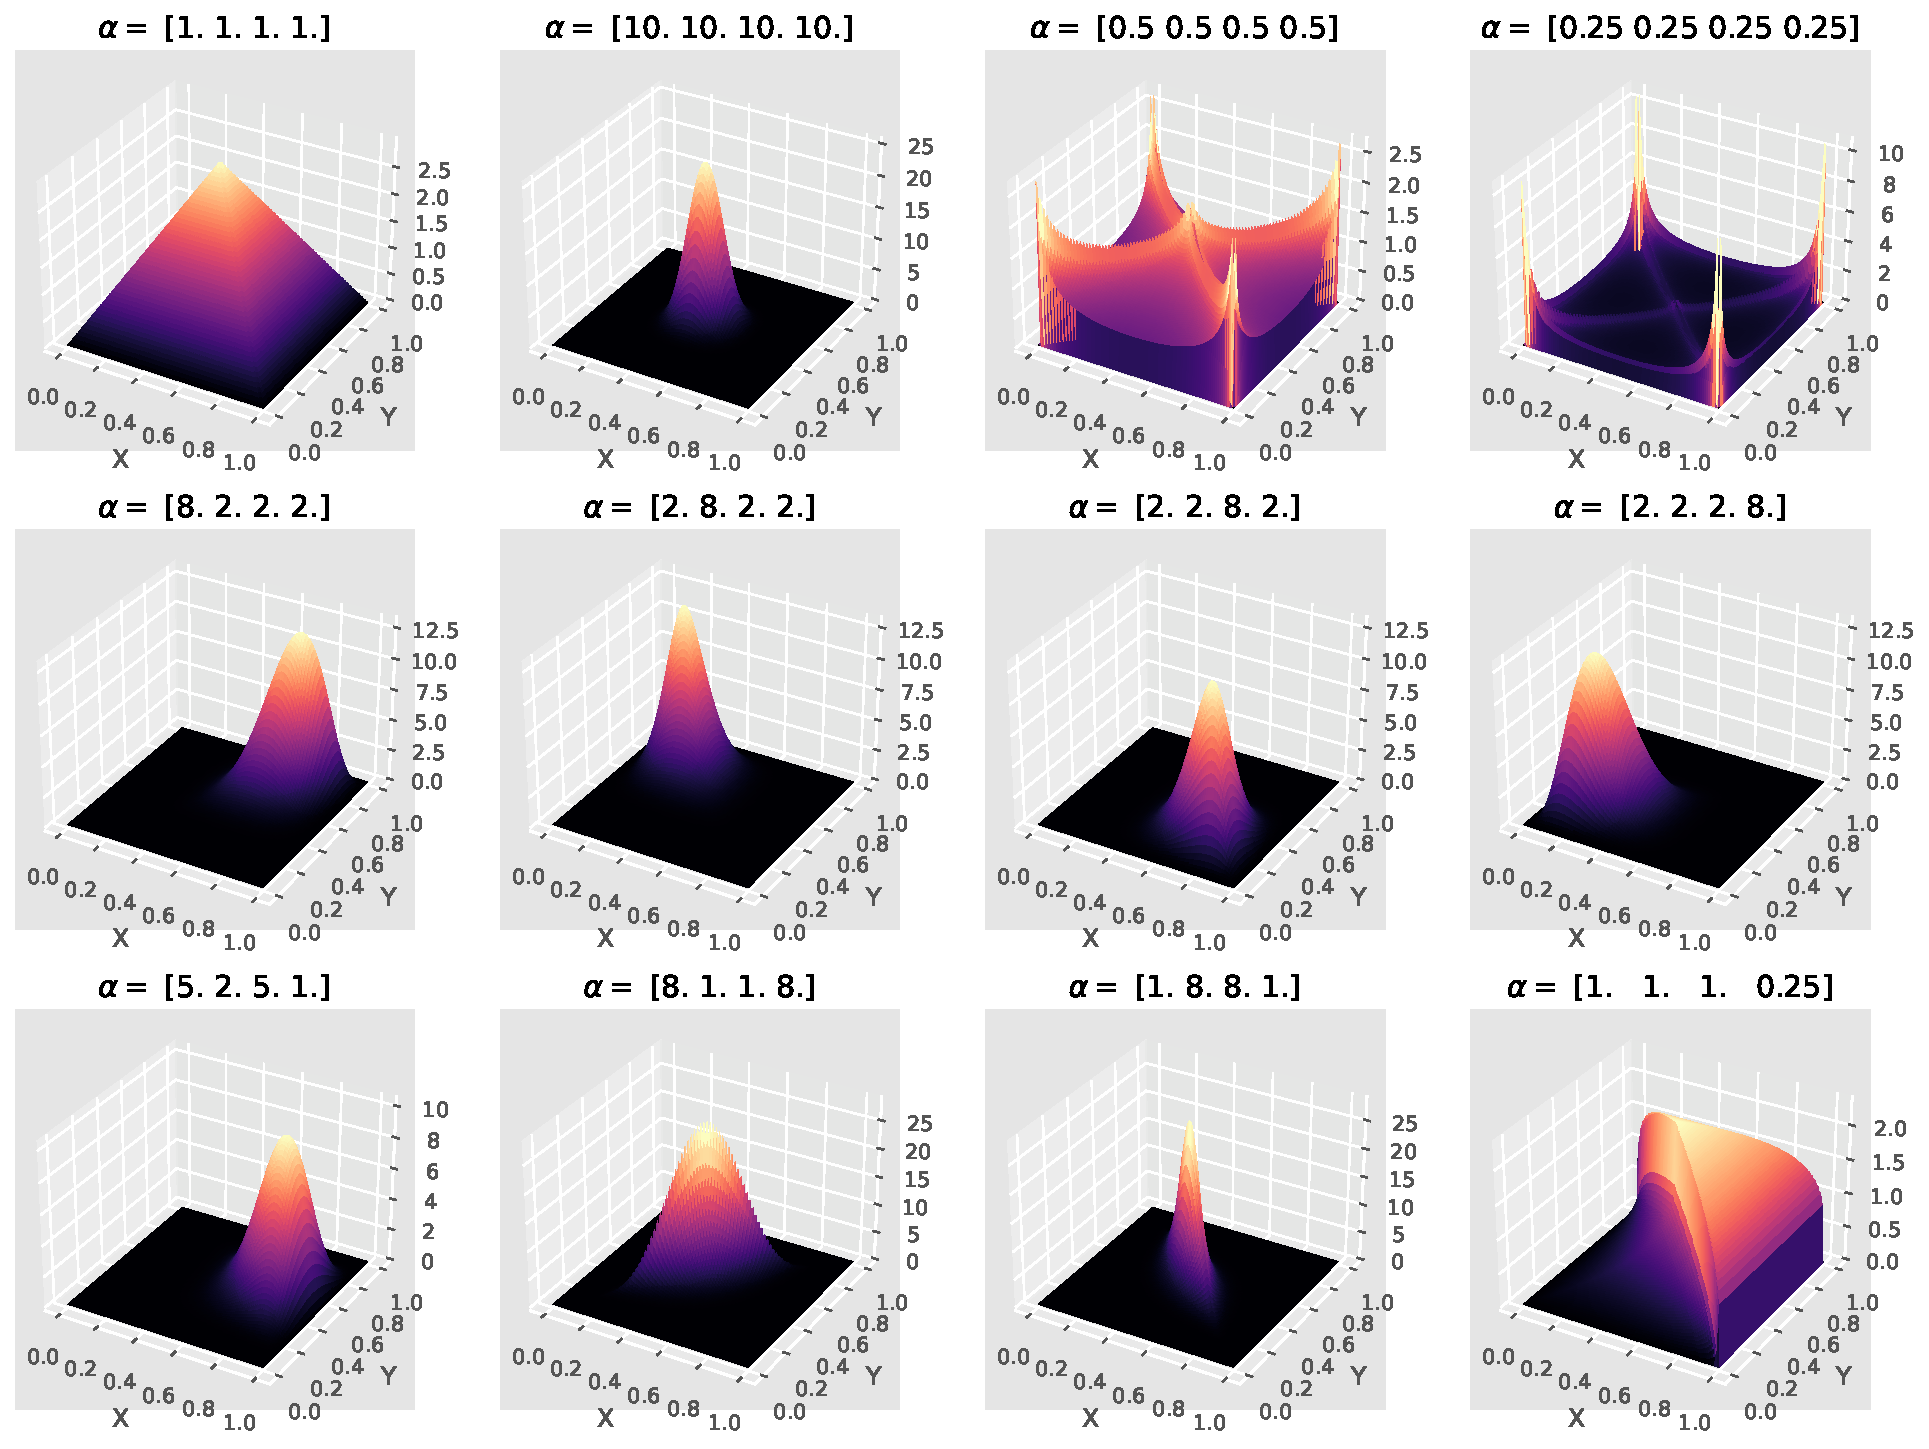
\includegraphics[width=14cm]{joint-densities-bivariate-beta.pdf}
  \fonte{Prepared by the author (2021). The four plots} in the first plot are
  symmetric and have no correlation between the variables. When $\alpha =
  [0.5, 0.5, 0.5, 0.5]$
  \label{fig:beta-bivariate}
\end{figure}

\begin{proposition}[Marginal distributions]
  \label{prop:marginal-distributions}
  The marginal distribution of $X$ is Beta with parameters $\alpha_1 +
  \alpha_2$ and $\alpha_3 + \alpha_4$. Similarly, the marginal distribution of
  $Y$ is Beta with parameters $\alpha_1 + \alpha_3$ and $\alpha_2 + \alpha_4$.
\end{proposition}

\begin{proof}
  First we derive the probability density of $(U_1, U_2)$.
  \begin{equation}
    \label{eq:dist-u1-u2}
    \begin{split}
      f_{U_1, U_2}(u_1, u_2) &= \int_{-\infty}^{\infty} f_{U}(u_1,u_2,u_3) \, du_3 \\ 
      &= \frac{1}{B(\boldsymbol{\alpha})}\int_0^1 u_1^{\alpha_1-1}u_2^{\alpha_2-1}u_3^{\alpha_3-1}(1-u_1-u_2-u_3)^{\alpha_4-1} \, du_3 \\
      &= \frac{1}{B(\boldsymbol{\alpha})}u_1^{\alpha_1-1}u_2^{\alpha_2-1}\int_0^1 u_3^{\alpha_3-1}(1-u_1-u_2-u_3)^{\alpha_4-1} \, du_3.
    \end{split}
  \end{equation}
  Let $u_3 = (1 - u_1 - u_2)z$. Then,
  \begin{equation}
    \begin{split}
      f_{U_1, U_2}(u_1, u_2) &= \frac{1}{B(\boldsymbol{\alpha})}u_1^{\alpha_1-1}u_2^{\alpha_2-1} \\
      &\hspace{1cm} \times \int_0^1 (1-u_1-u_2)^{\alpha_3-1}z^{\alpha_3-1}(1-u_1-u_2)^{\alpha_4}(1-z)^{\alpha_4-1} \, dz. \\
      &= \frac{1}{B(\boldsymbol{\alpha})}u_1^{\alpha_1-1}u_2^{\alpha_2-1}(1-u_1-u_2)^{\alpha_3+\alpha_4-1}\int_0^1 z^{\alpha_3-1}(1-z)^{\alpha_4-1} \, dz. \\
      &= \frac{1}{B(\boldsymbol{\alpha})}u_1^{\alpha_1-1}u_2^{\alpha_2-1}(1-u_1-u_2)^{\alpha_3+\alpha_4-1}\frac{\Gamma(\alpha_3)\Gamma(\alpha_4)}{\Gamma(\alpha_3 + \alpha_4)} \\
      &= \frac{1}{B(\alpha_1, \alpha_2, \alpha_3+\alpha_4)}u_1^{\alpha_1-1}u_2^{\alpha_2-1}(1-u_1-u_2)^{\alpha_3+\alpha_4-1}.
    \end{split}
  \end{equation}

We conclude that
$$(U_1, U_2, 1-U_1-U_2) \sim
\operatorname{Dirichlet}(\alpha_1,\alpha_2,\alpha_3+\alpha_4).$$

Define 
$$
H(v) = \begin{bmatrix}
  1 & 0 \\ 1 & 1
\end{bmatrix}v, \text{ for } v \in \R^2.
$$

Then $(U_1, X) = H(U_1, U_2)$ and $H(\cdot)$ is bijective and differentiable function. By the Change of Variable Formula, 
\begin{equation}
  \begin{split}
    f_{U_1, X}(u_1, x) &= f({H^{-1}(u_1,x)})\bigg|\det\left[\frac{dH^{-1}(v)}{dv}\bigg|_{v=(u_1,x)}\right]\bigg| \\ 
    &= f(u_1, x - u_1) = \frac{1}{B(\alpha_1, \alpha_2, \alpha_3+\alpha_4)}u_1^{\alpha_1-1}(x-u_1)^{\alpha_2-1}(1-x)^{\alpha_3+\alpha_4-1}, 
  \end{split}
\end{equation}
where $(u_1, x)$ belongs to the triangle defined by the points (0,0),
(0,1), and (1,1). The distribution of $X$ for $x \in [0,1]$ is
\begin{equation}
  \begin{split}
    f_X(x) &= \frac{1}{B(\alpha_1, \alpha_2, \alpha_3+\alpha_4)}\int_{0}^{x} u_1^{\alpha_1-1}(x-u_1)^{\alpha_2-1}(1-x)^{\alpha_3+\alpha_4-1} \, du_1 \\
    &= \frac{1}{B(\alpha_1, \alpha_2, \alpha_3+\alpha_4)}(1-x)^{\alpha_3+\alpha_4-1} \int_{0}^{x} u_1^{\alpha_1-1}(x-u_1)^{\alpha_2-1} \, du_1. \\
    &= \frac{1}{B(\alpha_1, \alpha_2, \alpha_3+\alpha_4)}(1-x)^{\alpha_3+\alpha_4-1} \\
    &\hspace{1cm}\times \int_{0}^{x} x^{\alpha_1-1} \left(\frac{u_1}{x}\right)^{\alpha_1-1}x^{\alpha_2 - 1}\left(1-\frac{u_1}{x}\right)^{\alpha_2-1} \, du_1. \\
  \end{split}
\end{equation}

Setting $u = u_1/x$ (if $x = 0, f_X(x) = 0$, then suppose $x > 0$), we have, 
\begin{equation}
  \begin{split}
    f_X(x) &= \frac{1}{B(\alpha_1, \alpha_2, \alpha_3+\alpha_4)}(1-x)^{\alpha_3+\alpha_4-1} x^{\alpha_1+\alpha_2-1} \int_{0}^{1} u^{\alpha_1-1}(1-u)^{\alpha_2-1} \, du. \\
    &= \frac{1}{B(\alpha_1, \alpha_2, \alpha_3+\alpha_4)}(1-x)^{\alpha_3+\alpha_4-1} x^{\alpha_1+\alpha_2-1} B(\alpha_1, \alpha_2)\\
    &= \frac{1}{B(\alpha_1 + \alpha_2, \alpha_3+\alpha_4)}(1-x)^{\alpha_3+\alpha_4-1} x^{\alpha_1+\alpha_2-1}\\
  \end{split}
\end{equation}
Therefore $X \sim \betadist(\alpha_1+\alpha_2, \alpha_3+\alpha_4)$. Similarly $Y \sim \betadist(\alpha_1+\alpha_3, \alpha_2 + \alpha_4)$.
\end{proof}

From the marginal distributions, we already know the expected values and variances of the random variables $X$ and $Y$. Denote $\tilde{\alpha} = \sum_{i=1}^4 \alpha_i$ and we have 

\begin{gather}
    \begin{aligned}
    \ev[X] &= \frac{\alpha_1 + \alpha_2}{\tilde{\alpha}},
    & \ev[Y] &= \frac{\alpha_1 + \alpha_3}{\tilde{\alpha}},
    \\
    \var[X] &= \frac{(\alpha_1 + \alpha_2)(\alpha_3 + \alpha_4)}{\tilde{\alpha}^2(\tilde{\alpha} + 1)},
    & \var[Y] &= \frac{(\alpha_1 + \alpha_3)(\alpha_2 + \alpha_4)}{\tilde{\alpha}^2(\tilde{\alpha} + 1)}.
    \end{aligned}
\end{gather}

\begin{proposition}[Bivariate beta density]
  \label{prop:bivariate-beta-density}
  The joint density of $(X,Y)$ with respect to the Lebesgue measure is
  given by 
  \begin{equation}
    f_{X,Y}(x,y) = \frac{1}{B(\boldsymbol{\alpha})}\int_{\Omega} u_1^{\alpha_1 - 1}(x - u_1)^{\alpha_2 -1}(y-u_1)^{\alpha_3-1}(1-x-y+u_1)^{\alpha_4-1} \, du_1,
  \end{equation}
  where 
  $$
  \Omega = (\max(0, x+y-1), \min(x,y)).
  $$
\end{proposition}

\begin{proof}
  Note that
  $$
  \begin{bmatrix}
    U_1 \\ X \\ Y
  \end{bmatrix}  = \begin{bmatrix}
    1 & 0 & 0 \\
    1 & 1 & 0 \\
    1 & 0 & 1
  \end{bmatrix}\begin{bmatrix}
    U_1 \\ U_2 \\ U_3
  \end{bmatrix}, 
  $$
  where the linear function is bijective and differentiable function, such
  that the determinant of the derivative is 1. By the Change of Variable
  Formula, 
  \begin{equation}
    \begin{split}
      f_{U_1,X,Y}(u_1,x,y) &= f_{U_1,U_2,U_3}(u_1, x - u_1, y - u_2) \\ 
      &= \frac{1}{B(\boldsymbol{\alpha})}u_1^{\alpha_1-1}(x-u_1)^{\alpha_2-1}(y-u_1 )^{\alpha_3-1}(1-x-y+u_1)^{\alpha_4-1},
    \end{split}
  \end{equation}
  where $0 \le u_1 \le x, u_1 \le y$, and $0 \le 1 - x - y + u_1$.  
  Hence,
  \begin{equation}
      \label{eq:dist-X-Y}
      f_{X,Y}(x,y) = \frac{1}{B(\boldsymbol{\alpha})}\int_{\Omega} u_1^{\alpha_1-1}(x-u_1)^{\alpha_2-1}(y-u_1)^{\alpha_3-1}(1-x-y+u_1)^{\alpha_4-1} \, du_1,
  \end{equation}
  such that $\Omega = \{u_1 : \max(0, x + y -1) < u_1 < \min(x,y)\}$.
\end{proof}

At last we derive the covariance and the correlation between $X$ and $Y$.

\begin{proposition}[Covariance and correlation]
  \label{prop:covariance-correlation}
  The covariance between $X$ and $Y$ is 
  $$\cov(X,Y) = \frac{1}{\tilde{\alpha}^2(\tilde{\alpha}+1)}(\alpha_1\alpha_4 - \alpha_2\alpha_3)$$
  and
  $$\cor(X,Y) = \frac{\alpha_1\alpha_4 - \alpha_2\alpha_3}{\sqrt{(\alpha_1+\alpha_2)(\alpha_3+\alpha_4)(\alpha_1+\alpha_3)(\alpha_2+\alpha_4)}}$$
\end{proposition}

\begin{proof}

  The covariance between $U_i$ and $U_j$ is \cite[p. 11]{lin2016dirichlet} 
\begin{equation}
  \cov(U_i, U_j) = - \frac{\alpha_i\alpha_j}{\tilde{\alpha}^2(\tilde{\alpha}+1)}, i,j = 1,...,4, i \neq j
\end{equation} 
and the variance of $U_i$ is 
\begin{equation}
  \var(U_i) = \frac{\alpha_i(\tilde{\alpha}-\alpha_i)}{\tilde{\alpha}^2(\tilde{\alpha}+1)},
\end{equation}
since $U_i \sim \operatorname{Beta}(\alpha_i, \tilde{\alpha} -\alpha_i)$.
Therefore 
\begin{equation}
  \cov(X,Y) = \cov(U_1+U_2, U_1+U_3) = \frac{1}{\tilde{\alpha}^2(\tilde{\alpha}+1)}(\alpha_1\alpha_4 - \alpha_2\alpha_3)
\end{equation}
  
\end{proof}

Now we present an example where the full range of correlation is covered.
Suppose $X$ and $Y$ have uniform distribution over $[0,1]$, that is, they have
beta distribution with parameter $1,1$. Then, we have that 
$$\alpha_1 +
\alpha_2 = \alpha_3 + \alpha_4 = \alpha_1 + \alpha_3 = \alpha_2 + \alpha_4 = 1,$$
whose solution is $\alpha_1 = \alpha_4 \in (0,1)$ and $\alpha_2 = \alpha_3 = 1
- \alpha_4$. The correlation formula boils down to 
$$\cor(X,Y) = \alpha_4^2 - (1 - \alpha_4)^2 = 2\alpha_4 - 1 \in (-1,1).$$

\section{Implementation of the dirichlet distribution in Stan}

The Dirichlet distribution is defined on the simplex of lower dimension.
Therefore the sampler has to consider the restriction of $\sum_{i=1}^4 U_i =
  1$. \textcite{betancourt2012cruising} presents a simplification in the
structure of the simplex. The propose is \cite[p. 2]{betancourt2012cruising}
\begin{equation*}
  \begin{aligned}
    z_i & \sim \betadist(\tilde{\alpha}_i, \alpha_i), \text{ where } \tilde{\alpha}_i = \sum_{k=i+1}^4 \alpha_k, \quad i = 1,2,3 \\
    U_i & = \left(\prod_{k=1}^{i-1} z_k\right)\cdot \begin{cases}
      1 - z_i, & i < 4 \\
      1,       & i = 4
    \end{cases},
  \end{aligned}
\end{equation*}
which removes the constraint.

\section{Comments about integration}

The density of $(X,Y)$ is $f_{X,Y}(x,y)$ as in equation \eqref{eq:dist-X-Y}. Therefore it can be undefined in sets of null Lebesgue measure in $\R^2$ and these sets may be important when plotting in a grid, for instance. This section illustrates one of these sets. If $\alpha_i \ge 1,
\, i = 1,...,4$, the integral is clearly well defined for every $x,y \in [0,1]$. Let $0 < \alpha_2 = \alpha_3 = a \le 0.5$ and $x = y < 0.5$. Then
\begin{equation*}
  \begin{split}
    f_{X,Y}(x,y) &= \frac{1}{B(\boldsymbol{\alpha})}\int_{0}^x u_1^{\alpha_1-1}(x-u_1)^{a-1}(x-u_1)^{a-1}(1-2x+u_1)^{\alpha_4-1} \, du_1 \\
    &= \frac{1}{B(\boldsymbol{\alpha})}\int_{0}^{x/2} u_1^{\alpha_1-1}(x-u_1)^{2a-2}(1-2x+u_1)^{\alpha_4-1} \, du_1 + \\
    &~~~+ \frac{1}{B(\boldsymbol{\alpha})}\int_{x/2}^x u_1^{\alpha_1-1}(x-u_1)^{2a-2}(1-2x+u_1)^{\alpha_4-1} \, du_1
  \end{split}
\end{equation*}

Note that the first integral is well defined and non-negative. On the other hand, the second integral is not defined: 
\begin{equation*}
  \begin{split}
    \int_{x/2}^{x} u_1^{\alpha_1-1}&(x-u_1)^{2a-2}(1-2x+u_1)^{\alpha_4-1} \, du_1 \\
    &\ge \int_{x/2}^x \min\left(\left(\frac{x}{2}\right)^{\alpha_1-1}, x^{\alpha_1-1}\right)(x-u_1)^{2a-2} \\ 
    &\hspace{3cm} \times \min\left(\left(1-\frac{3}{2}x\right)^{\alpha_4-1}, (1-x)^{\alpha_4-1}\right) \, du_1 \\
    &= K(x) \int_{0}^{x/2} v^{2a-2} \, dv \\ 
    &= \begin{cases}
      \dfrac{K(x)}{2a-1} \lim_{t \to 0^+} \left[(x/2)^{2a-1} - t^{2a-1}\right] &\text{ if } a < 0.5 \\ 
      K(x) \lim_{t \to 0^+} \left[\log(x/2) - \log(t)\right] &\text{ if } a = 0.5
    \end{cases} \\
    &\to +\infty, 
  \end{split}
\end{equation*}
where $K(x)$ is a function of $x$. 

Based on this divergence, we conclude that if $0 < \alpha_2 = \alpha_3 \le 0.5$
and $x = y < 0.5$, $f_{X,Y}(x,y)$ is not defined. Notice that if $x = y \ge
0.5$, divergence problems still happens, since the problems appear when $u_1$ approximates $x$. Similar calculations show that if $x + y = 1$ and $0 < \alpha_1 = \alpha_4 \le 0.5$, the density is also
not defined. More generally, $f_{X,Y}(x,y)$ is not defined if $\alpha_1 +
\alpha_4 \le 1$ and $x + y = 1$; $\alpha_2 + \alpha_3 \le 1$ and $x = y$.

\section{Elicitation of a bivariate beta}
\label{sec:elicitation-bivariate-beta}

In this section, we develop a method to elicit the parameters of the bivariate
beta distribution, which means to define an approximation
$\hat{\boldsymbol{\alpha}}$ for the parameter $\boldsymbol{\alpha}$. 
This is an important step for the characterization of the prior distribution of model
\eqref{model:sensitivity-specificity}. If the researcher does not have
information about the parameters previous seeing the data, two approaches
are common in the independent beta setting and are adapted for the bivariate 
case:

\begin{alineas}
  \item both parameters receive a uniform distribution: in this case, as
  mentioned in Proposition \ref{prop:covariance-correlation}, $\alpha_1 =
  \alpha_4 \in (0,1)$ and $\alpha_2 = \alpha_3 = 1 - \alpha_4$. The parameter
  $\alpha_4$ is defined in a way that $\alpha_4 = \frac{1}{2}(1 + \cor(X,Y))$.
  If no information about the variables' correlation is available, it is recommended to use
  the independent setting since it is more flexible;
  \item both parameters receive a Jeffreys prior distribution
  ($\betadist(1/2,1/2)$): in this case,  $\alpha_1 =
  \alpha_4 \in (0,1/2)$ and $\alpha_2 = \alpha_3 = 1 - \alpha_4$. The parameter
  $\alpha_4$ is defined in a way that $\alpha_4 = \frac{1}{4}(1 + \cor(X,Y))$.
\end{alineas}

Now, suppose that the researcher has information about following moments of
the bivariate beta distribution: $m_1 = \ev[X], m_2 = \ev[Y], v_1 = \var(X),
v_2 = \var(Y)$, and $\rho  = \cor(X,Y)$. Notice that $v_1 + m_1^2 = \var(X_1)
+ \ev[X_1]^2 = \ev[X_1^2]$ and
$$
\ev[X_1^2] - \ev[X_1] = \frac{(\alpha_1 + \alpha_2 + 1)(\alpha_1 + \alpha_2)}{(\tilde{\alpha} + 1)\tilde{\alpha}} - \frac{\alpha_1 + \alpha_2}{\tilde{\alpha}} = -\frac{(\alpha_1 + \alpha_2)(\alpha_3 + \alpha_4)}{\tilde{\alpha}(\tilde{\alpha}+1)} < 0, 
$$
that is, $v_1 + m_1^2 - m_1 < 0 \implies v_1 < m_1 - m_1^2$ and similarly,
$v_2 < m_2 - m_2^2$. After fixing these quantities, we will have a non-linear system with five equations and four
unknown variables. Hence, we want to solve the following 
\begin{equation}
  \label{eq:system-moments-alpha}
  \begin{cases}
    m_1 = \dfrac{\alpha_1+\alpha_2}{\tilde{\alpha}} \\
    m_2 = \dfrac{\alpha_1+\alpha_3}{\tilde{\alpha}} \\ 
    v_1 = \dfrac{(\alpha_1+\alpha_2)(\alpha_3+\alpha_4)}{\tilde{\alpha}^2(\tilde{\alpha}+1)} \\
    v_2 = \dfrac{(\alpha_1+\alpha_3)(\alpha_2+\alpha_4)}{\tilde{\alpha}^2(\tilde{\alpha}+1)} \\
    \rho = \dfrac{\alpha_1\alpha_4 - \alpha_2\alpha_3}{\sqrt{(\alpha_1+\alpha_2)(\alpha_3+\alpha_4)(\alpha_1+\alpha_3)(\alpha_2+\alpha_4)}}
  \end{cases}
\end{equation}

Notice that we can simplify the third and fourth equations since 
$$
\frac{\alpha_3 + \alpha_4}{\tilde{\alpha}} = \frac{\tilde{\alpha} - (\alpha_1 + \alpha_2)}{\tilde{\alpha}} = 1 - m_1 
$$
and analogously, 
$$
\frac{\alpha_2 + \alpha_4}{\tilde{\alpha}} = 1 - m_2. 
$$
Therefore, 
\begin{align*}
    v_1 &= \frac{m_1(1 - m_1)}{\tilde{\alpha} + 1} \\
    v_2 &= \frac{m_2(1 - m_2)}{\tilde{\alpha} + 1}
\end{align*}

This already tells us that the system do not have a solution if 
$$
\frac{m_1(1-m_1)}{v_1} \neq \frac{m_2(1-m_2)}{v_2}. 
$$

The following proposition builds a solution excluding the fourth equation, given the above comment. 

\begin{proposition}
  \label{prop:solution-to-system-bivariate-beta}
  System \eqref{eq:system-moments-alpha} without the fourth equation has a unique solution given by 
\begin{gather}
 \label{eq:system-solution}
 \begin{aligned}
  \alpha_1 &= (m_1 + m_2 - 1)\tilde{\alpha} + \alpha_4 \\
  \alpha_2 &=  (1 - m_2)\tilde{\alpha} - \alpha_4 \\
  \alpha_3 &= (1-m_1)\tilde{\alpha} - \alpha_4. \\
  \alpha_4 &= \rho\tilde{\alpha}\sqrt{m_1m_2(1-m_1)(1-m_2)} + (1-m_1)(1-m_2),
\end{aligned}
\end{gather}
where $\tilde{\alpha}$ is given by the expression 
$$
\tilde{\alpha} = \frac{(m_1 - m_1^2 - v_1)}{v_1}.
$$
\end{proposition}

\begin{proof}
  The first two equations of the system \eqref{eq:system-moments-alpha} can be
rewritten as a linear system:
\begin{align*}
  (m_1 - 1)\alpha_1 + (m_1 - 1)\alpha_2 + m_1\alpha_3 + m_1\alpha_4 &= 0 \\
  (m_2 - 1)\alpha_1 + m_2\alpha_2 + (m_2-1)\alpha_3 + m_2\alpha_4 &= 0,   
\end{align*}
which is equivalent to 
\begin{align*}
  \alpha_1 + \alpha_2 + \frac{m_1}{m_1-1}\alpha_3 + \frac{m_1}{m_1-1}\alpha_4 &= 0 \\
  \alpha_2 + \frac{1-m_2}{m_1-1}\alpha_3 + \frac{m_1-m_2}{m_1-1}\alpha_4 &= 0.
\end{align*}
Then, we can write $\alpha_1$ and $\alpha_2$ as functions of $\alpha_3$ and
$\alpha_4$:
\begin{align}
  \label{eq:alpha1-as-function-alpha3-alpha4}
  \alpha_1 &= \frac{m_1+m_2-1}{1-m_1}\alpha_3 + \frac{m_2}{1-m_1}\alpha_4 \\
  \label{eq:alpha2-as-function-alpha3-alpha4}
  \alpha_2 &= \frac{1-m_2}{1-m_1}\alpha_3 + \frac{m_1-m_2}{1-m_1}\alpha_4.
\end{align}

Based on that expression, denote $\alpha_1 = a_3\alpha_3 + a_4\alpha_4$, $\alpha_2
= b_3\alpha_3 + b_4\alpha_4$, $c_3 = a_3 + b_3 + 1$, and $c_4 = a_4 + b_4 + 1$. Then, the third equation can be written as 
$$
a_3\alpha_3 + a_4\alpha_4 + b_3\alpha_3 + b_4\alpha_4 + \alpha_3 + \alpha_4 + 1 = c_3\alpha_3 + c_4 \alpha_4 = \frac{m_1(1-m_1)}{v_1} - 1, 
$$
which implies that 
$$
\alpha_3 = \frac{m_1(1-m_1) - v_1 - c_4v_1\alpha_4}{c_3v_1},
$$
that is a linear function of $\alpha_4$. We summarize the expressions in function of $\alpha_4$ with some simplifications: 
\begin{align*}
  \alpha_1 &= (m_1 + m_2 - 1)\frac{(m_1 - m_1^2 - v_1)}{v_1} + \alpha_4 \\
  \alpha_2 &=  (1 - m_2)\frac{(m_1 - m_1^2 - v_1)}{v_1} - \alpha_4 \\
  \alpha_3 &= (1-m_1)\frac{(m_1 - m_1^2 - v_1)}{v_1} - \alpha_4,
\end{align*}
which implies that 
$$
\tilde{\alpha} = \frac{m_1 - m_1^2 - v_1}{v_1}.
$$

Now rewrite the fifth equation using the first two equations from system \eqref{eq:system-moments-alpha} as follows 
\begin{equation}
    \label{eq:rho-equation}
    \begin{split}
        \rho &= \frac{\alpha_1\alpha_4 - \alpha_2\alpha_3}{\sqrt{(\alpha_1+\alpha_2)(\alpha_3+\alpha_4)(\alpha_1+\alpha_3)(\alpha_2+\alpha_4)}} \\ 
        &= \frac{\alpha_1\alpha_4 - \alpha_2\alpha_3}{\tilde{\alpha}^2\sqrt{m_1m_2(1-m_1)(1-m_2)}} \\ 
        &= \frac{(m_1 + m_2 - 1)\tilde{\alpha}\alpha_4 + \alpha_4^2 - ((1-m_2)\tilde{\alpha} - \alpha_4)((1-m_1)\tilde{\alpha} - \alpha_4)}{\tilde{\alpha}^2\sqrt{m_1m_2(1-m_1)(1-m_2)}} \\
        &= \frac{\alpha_4 - (1-m_1)(1-m_2)\tilde{\alpha}}{\tilde{\alpha}\sqrt{m_1m_2(1-m_1)(1-m_2)}} \\ 
    \end{split}
\end{equation}
and the solution is, therefore, 
$$
\alpha_4 = \rho\tilde{\alpha}\sqrt{m_1m_2(1-m_1)(1-m_2)} + (1-m_1)(1-m_2).
$$
\end{proof}

There is an additional restriction to the sum given by the marginal
distributions. Let $Z \sim \betadist(a, b)$. Then: 
$$
\frac{\ev[Z](1-\ev[Z])}{\var[Z]} - 1 = \frac{\frac{ab}{(a+b)^2}}{\frac{ab}{(a+b)^2(a+b+1)}}-1 = a+b, 
$$
then 
\begin{equation}
  \label{eq:restriction-sum-alphas}
  \sum_{i=1}^4 \alpha_i = \frac{m_1(1-m_1)}{v_1} - 1 = \frac{m_2(1-m_2)}{v_2} - 1.
\end{equation}

Besides solving the system \eqref{eq:system-moments-alpha}, the bivariate 
beta distribution needs that $\alpha_1, \dots, \alpha_4 > 0$. However, this is not necessarily
true. Since it is difficult to find the subset $D \subset [0,1]^4$ in which
the solution for \eqref{eq:system-solution} is strictly positive for
$\alpha_1, \dots, \alpha_4$, we present some examples in Figure
\ref{fig:alpha-solutions}. For each subplot, the values of $v_1$ and $\rho$
are fixed, while $m_1, m_2 \in [0,1]^2$. The grey area corresponds to the set 
where $v_1 \ge m_1 - m_2$, which is impossible. The orange area means that
the solution to system \eqref{eq:system-moments-alpha} is not strictly
positive. At last, the blue region is the set of interest. 

When $\rho = -1$ for instance, only a few specifications of $m_1$ and $m_2$
generate a strictly positive solution. These examples show that several
interesting specifications for the researchers can lead to a non positive
solution, which is not desirable. 

\begin{figure}[!ht]
    \centering
    \caption{Verification of positivity of the solution for different and
    fixed values of $v_1$ and $\rho$, and $m_1, m_2 \in [0,1]^2$.} 
    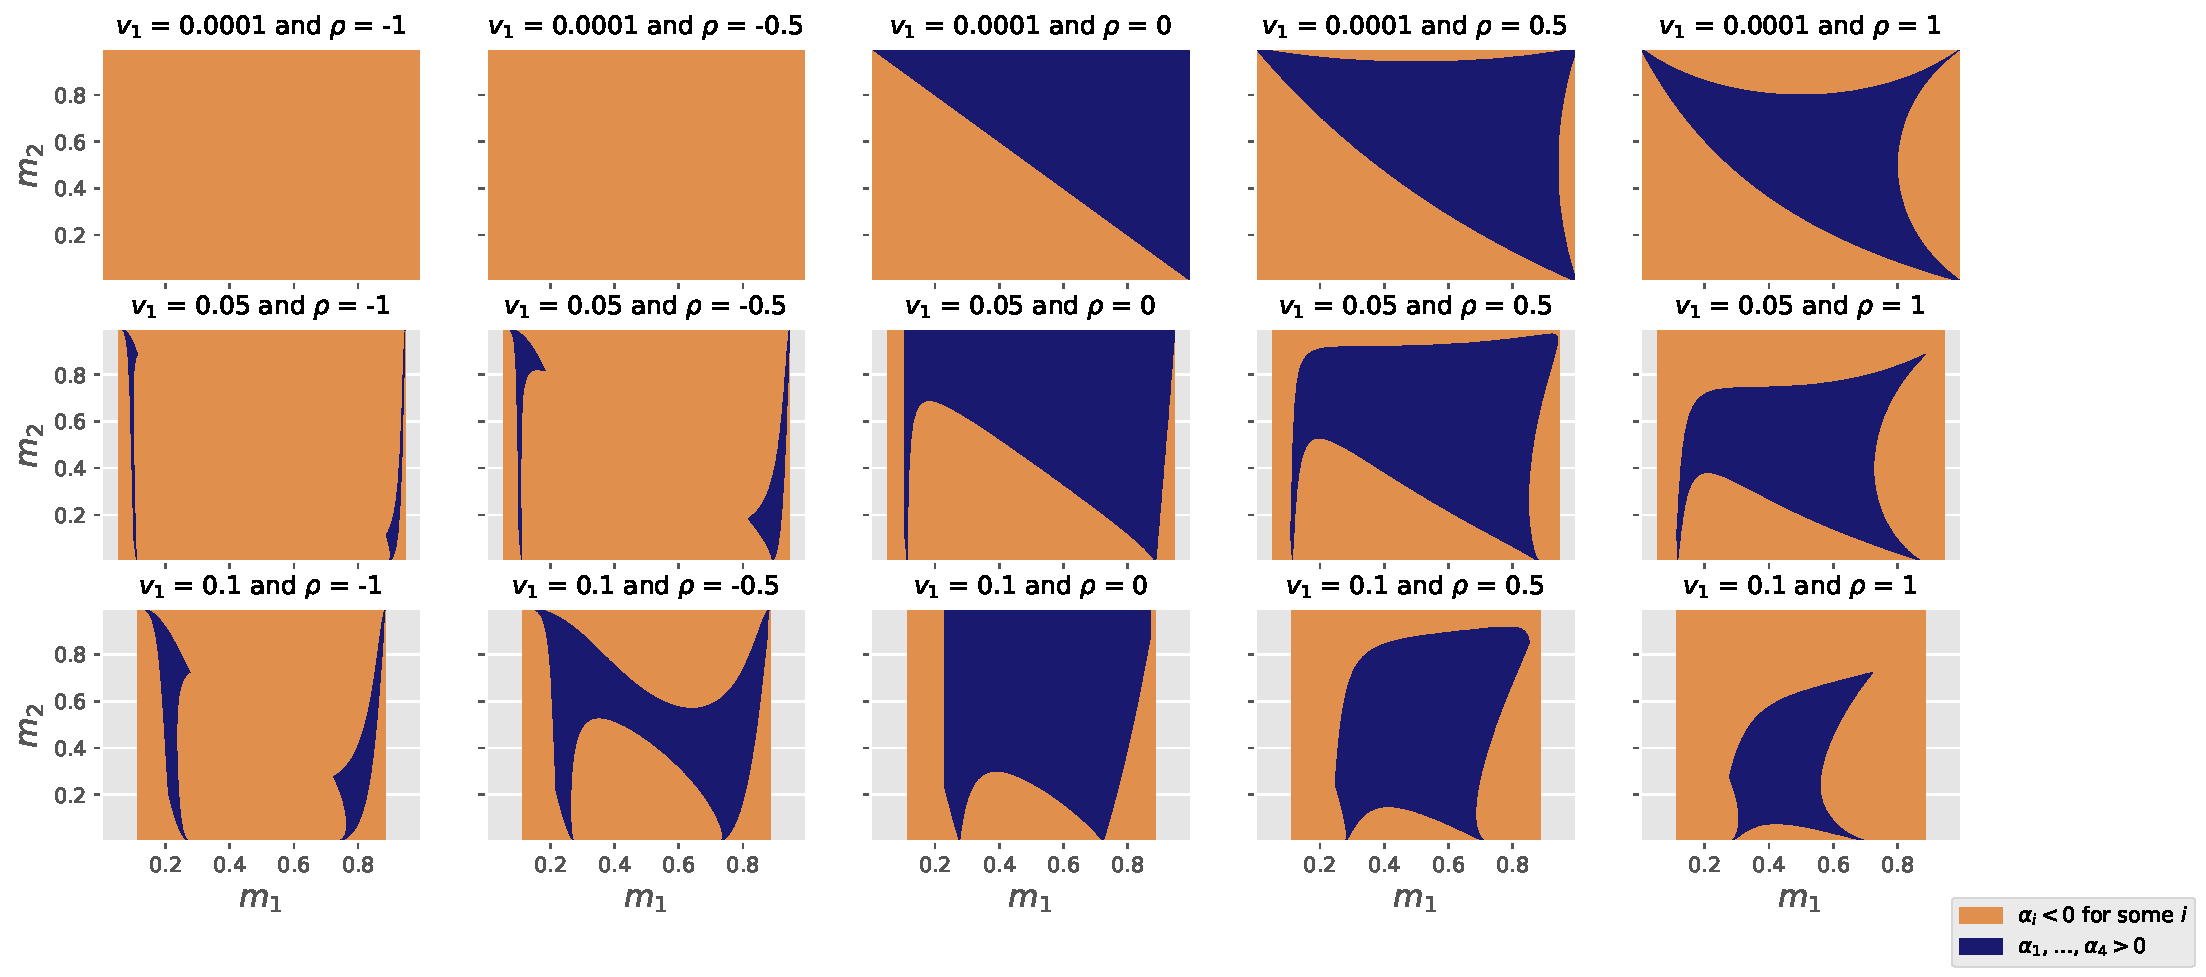
\includegraphics[width=\textwidth]{alpha_solution_existence.pdf}
    \fonte{Prepared by the author (2021).}
    \label{fig:alpha-solutions}
\end{figure}

Because of that reason, we can only have an approximation using some
optimization solver. From now on we suppose the researcher has knowledge about
$m_1$, $m_2$ and $\rho$. Through equations
\eqref{eq:alpha1-as-function-alpha3-alpha4}, 
\ref{eq:alpha2-as-function-alpha3-alpha4}, and solving the correlation
equation for $\alpha_3$ with help of the symbolic solver SymPy \cite{sympy},
we have the following three expressions: 
\begin{equation*}
  \begin{aligned}
    \alpha_1 &= \alpha_4\frac{m_1m_2 + \rho\sqrt{m_1m_2(1-m_1)(1-m_2)}}{(1-m_1)(1-m_2) + \rho\sqrt{m_1m_2(1-m_1)(1-m_2)}} \\
    \alpha_2 &= \alpha_4\frac{m_1(1-m_2) - \rho\sqrt{m_1m_2(1-m_1)(1-m_2)}}{(1-m_1)(1-m_2) + \rho\sqrt{m_1m_2(1-m_1)(1-m_2)}} \\
    \alpha_3 &= \alpha_4\frac{m_2(1-m_1) - \rho\sqrt{m_1m_2(1-m_1)(1-m_2)}}{(1-m_1)(1-m_2) + \rho\sqrt{m_1m_2(1-m_1)(1-m_2)}},
  \end{aligned}
\end{equation*}
and $\alpha_4 > 0$ is a free parameter. In order to have $\boldsymbol{\alpha} >
0$, we have two situations:
\begin{alineas}
  \item the denominador of $\alpha_1, \alpha_2, \alpha_3$ is negative: in this
  case, it is not possible to have both $\alpha_2$ and $\alpha_3$ positives;
  \item the denominador of  $\alpha_1, \alpha_2, \alpha_3$ is positive: in
  this case, we have that 
  $$
  \rho \in \left(-\frac{\min(m_1m_2, (1-m_1)(1-m_2))}{\sqrt{m_1m_2(1-m_1)(1-m_2)}}, 
  \frac{\max(m_1, m_2) - m_1m_2}{\sqrt{m_1m_2(1-m_1)(1-m_2)}}\right).
  $$
\end{alineas}

When $m_1 = m_2 = m$, the upper bound is 1 and the lower bound is 
$$\begin{cases}
  -\dfrac{m}{1-m}, &m < 1/2 \\
  -\dfrac{1-m}{m}, &m > 1/2.
\end{cases}$$

Suppose that $\rho$ belongs to this interval. Then we have to choose $\alpha_4
> 0$. Using a symbolic solver, we see that 
$$
\sum_{i=1}^4 \alpha_i = \frac{\alpha_4}{(1-m_1)(1-m_2) + \rho\sqrt{m_1m_2(1-m_1)(1-m_2)}}, 
$$
therefore $v_1$ and $v_2$ are inversely proportional to $\alpha_4$. To have a
higher variance, pick a small $\alpha_4$. To have a lower variance, pick a
large one. If $\rho$ does not belong to the interval, taking a suitable value
in it is a possibility. 

Suppose the researcher has also knowledge about $v_1$ and $v_2$. By
Proposition \ref{prop:solution-to-system-bivariate-beta} and
\autoref{fig:alpha-solutions}, there is no viable
solution in several situations. Because of that, two approaches are suggested:

\begin{alineas}
  \item no variable is fixed: solve the optimizing problem given by 
  \textcite[p. 7]{olkin2015constructions}. The problem with this approach is 
  that $\rho$ and the means $m_1, m_2$ get distanced from the given values.
  Weights can be specified for each parameter to incorporate some preference;  
  \item fix $m_1$ and $m_2$ and let $\rho, v_1$ and $v_2$ vary: it is the
  limit of the above method, with the weights of $m_1$ and $m_2$ going to the
  infinity. It is more suitable when the researcher has more beliefs in the
  means than the other moments. 
\end{alineas}

In this work, we use the second approach, which give less importance to the
correlation in comparison to the means. 

\begin{remark}
  If the researcher has information about a credibility interval, this
  information needs to be converted in terms of the variance.
\end{remark}

\section{Simulate data}

In this section we experiment the estimation process of $\hat{\boldsymbol{\alpha}}$ through
two different simulations: 

\begin{alineas}
  \item simulating from bivariate beta: fix the parameter $\alpha = (0.5, 0.5,
  0.5, 0.5)$ and generate $1000$
  different datasets from bivariate beta distribution of size $100$; calculate
  $m_1, m_2, v_1, v_2$, and $\rho$ and (i) solve the equations through Proposition
  \eqref{prop:solution-to-system-bivariate-beta}, (ii) complete optimization
  problem, and (iii) optimization problem with $m_1$ and $m_2$ fixed, which we
  call {\em mixed solver}. The mean squared error is calculated;
  \item simulating from bivariate logit normal distribution: fix the means and
  covariance matrix and follow the same instructions from the previous item.
\end{alineas}

Since the comparison is in terms of mean squared error, it is clear that the
minimization problem will have the least value. When time is important, it is
a very expensive method. Solving equations should be the best method, but
under uncertainty, its results can have biases.
\autoref{tab:comparing-approaches-bivariate-beta} summarizes the results. 
Notice that when simulating from the bivariate beta or from the bivariate
logit normal with parameters corresponding to the beta, the estimation process
has little error. 

\begin{table}[hb]
  \centering
  \caption{\label{tab:comparing-approaches-bivariate-beta}Comparing the
  different methods for each simulation strategy.}
  \begin{tabular}{cccc}
  \hline
  \multicolumn{1}{c}{\textbf{Simulation}} & \textbf{Method} & \textbf{MSE} & \textbf{s/ite} \\ \hline
  \multirow{3}{*}{Bivariate beta} & Solving equations & 0.04 & $3.47 \cdot 10^{-5}$ \\
   & Minimization problem & 0.032 & $1.43$ \\
   & Mixed solver & 0.033 & $0.03$ \\
  \multirow{3}{*}{Logit bivariate normal} & Solving equations & 0.034 & $5.21 \cdot 10^{-5}$ \\
   & Minimization problem & 0.026 & $1.53$ \\
   & Mixed solver & 0.026 & $0.03$  \\ \hline
  \end{tabular}
  \fonte{Prepared by the author (2021). The MSE is the mean squared error,
  where the mean is taken with respect to the iterations. The s/ite is the
  number of seconds per iteration.}
\end{table}

Using the logit bivariate normal simulation with parameters $\mu = (5, 2.3)$
and $\Sigma = [[12, -2.5], [-2.5, 4]]$ in order to yield $\ev[X] \approx 0.9,
\ev[Y] \approx 0.8, \var(X) = \var(Y) \approx 0.05$, and $\cor(X,Y) \approx
-0.2$, 77\% of the simulations has no exact solution strictly positive and the
error of the solvers were 0.82 for the mixed solver and 0.91 for the
minimization problem, which is much higher than the previous simulation.

\chapter{Sampling from the posterior distribution of the graph}
\label{sec:sampling-posterior-graph}

Here we derive the method developed by \textcite{crawford2016} for sampling
from $p(G_S, \lambda \mid \boldsymbol{Z})$. The
implementation used Python language. We first define
the prior density for $(G_s, \lambda)$ as 
$$
\pi(G_S, \lambda) = \pi(G_S) \times \pi(\lambda) = \frac{1}{|\mathcal{C}(\boldsymbol{Z})|} \times \frac{\beta_{r}^{\alpha_{r}}}{\Gamma(\alpha_{r})}\lambda^{\alpha_r - 1}e^{-\beta_r \lambda}, 
$$
where $\alpha_r$ and $\beta_r$ are positive hyperparameters. Notice that $G_S$
as uniform distribution over all compatible graphs and $\lambda \sim
\operatorname{Gamma}(\alpha_r, \beta_r)$.

To perform Gibbs sampling, we need to sample from $p(G_S \mid \lambda,
\boldsymbol{Z})$ and $p(\lambda \mid G_S , \boldsymbol{Z})$. Since we do not
know to sample from both conditional distributions, \textcite{crawford2016}
proposes to use Metropolis-Hastings for each one. Then, we need to specify a
proposal distribution to both conditionals:
\begin{alineas}
  \item the proposal for $p (G_S | \lambda, \boldsymbol{Z})$ generates a new compatible graph
   $G_S^*$ with a simple algorithm. It samples two random nodes $i,j$
   without replacement. If both nodes have less connections in $G_S$ than
   their informed degrees, i.e., $u_i \ge 1$ and
   $u_j \ge 1$, and they are not connected in $G_S$, we include the edge
   $\{i,j\}$ in $G_S^*$ and copy all the other edges. If the edge already is
   in $G_S$ and it is not in $G_R$, we remove it from $G_S^*$. Otherwise we
   draw another two nodes and continue. We call this proposal of $P(G_S^* \mid
   G_S)$; 
   \item the proposal for $p(\lambda \mid G_S, \boldsymbol{Z})$ assumes a
   normal distribution for the Maximum likelihood estimator (MLE)
   $\hat{\lambda}$ of $\lambda$ from the likelihood
   \eqref{eq:likelihood-wainting-times}. Deriving it, we obtain 
   \begin{equation*}
     \begin{split}
      \frac{d}{d \lambda} \log L(w \mid G_S, \lambda) &= \frac{d}{d \lambda}\left[ (n - m)\log(\lambda) + \sum_{k \mathrm{isn't seed}} \log(s_k) - \lambda \boldsymbol{s}^Tw\right] \\
      &= \frac{n-m}{\lambda} - \boldsymbol{s}^Tw,
     \end{split}
   \end{equation*}
   where $m$ is the number of seeds. At the optimal $\hat{\lambda}$, we have
   that 
   $$
   \frac{n-m}{\hat{\lambda}} - \boldsymbol{s}^Tw = 0 \implies \hat{\lambda} = \frac{n-m}{\boldsymbol{s}^Tw}.
   $$
   The Fisher information is, under some regularity conditions,
   $$
   I(\lambda) = -\ev\left[-\frac{n-m}{\lambda^2}\right] = \frac{n-m}{\lambda^2}.
   $$
   For a large $n$, we can assume
   $$\sqrt{n-m}(\hat{\lambda} - \lambda) \overset{d}{\to} N(0, \lambda^2).$$ 
   Then the proposal distribution is the normal distribution of mean
   $\hat{\lambda}$ and variance $\sigma^2 = \lambda^2/(n - m)$.
\end{alineas} 

Now, it remains to calculate the probability of acceptance for both
Metropolis-Hastings samplings. \textcite{crawford2016} 
establishes several results to make the calculations more efficient. We omit
then here. Using relation \eqref{eq:alpha-metropolis-hastings}, the probabilities are: 

\begin{alineas}
  \item for the graph transition:
  \begin{equation*}
    \begin{split}
      \alpha(G_S^* \mid G_S) &= \min\left(1, \frac{p (G_S^*| \lambda, \boldsymbol{Z})P(G_S \mid G_S^*)}{p (G_S | \lambda, \boldsymbol{Z}) P(G_S^* \mid G_S)}\right) \\
      &= \min\left(1, \frac{L(w \mid G_S^*, \lambda)\pi(G_S^*)\pi(\lambda)P(G_S \mid G_S^*)}{ L(w \mid G_S, \lambda)\pi(G_S)\pi(\lambda)P(G_S^* \mid G_S)}\right) \\
      &= \min\left(1, \frac{L(w \mid G_S^*, \lambda)P(G_S \mid G_S^*)}{ L(w \mid G_S, \lambda)P(G_S^* \mid G_S)}\right);
    \end{split}
  \end{equation*}
  \item for the rate $\lambda$ transition:
  \begin{equation*}
    \begin{split}
      \alpha(\lambda^* \mid \lambda) &= \min\left(1, \frac{p (\lambda^* \mid  G_S,  \boldsymbol{Z})g(\lambda \mid G_S)}{p (\lambda \mid G_S, \boldsymbol{Z}) g(\lambda^* \mid G_S)}\right) \\
      &= \min\left(1, \frac{L(w \mid G_S, \lambda^*)\pi(G_S)\pi(\lambda^*)g(\lambda \mid G_S)}{ L(w \mid G_S, \lambda)\pi(G_S)\pi(\lambda)P(\lambda \mid G_S)}\right) \\
      &= \min\left(1, \frac{L(w \mid G_S, \lambda^*)\pi(\lambda^*)g(\lambda \mid G_S)}{ L(w \mid G_S, \lambda)\pi(\lambda) g(\lambda^* \mid G_S)}\right).
    \end{split}
  \end{equation*}
  This probability is better calculated using the logarithmic transformations,
  since 
  $$
  \log \frac{L(w \mid G_S, \lambda^*)}{ L(w \mid G_S, \lambda)} = (n-m)\left(\log(\lambda^*) - \log(\lambda)\right) - \boldsymbol{s}^Tw(\lambda^* - \lambda),
  $$
  $$
  \log \frac{\pi(\lambda^*)}{\pi(\lambda)} = (\alpha_r - 1)(\log(\lambda^*) - \log(\lambda)) - \beta(\lambda^* - \lambda), \text{ and }
  $$
  $$
  \log \frac{g(\lambda \mid G_S)}{g(\lambda^* \mid G_S)} = \log(\lambda^*) - \log(\lambda) - \frac{1}{2}\left[\frac{(\lambda - \hat{\lambda})^2}{\sigma^2} - \frac{(\lambda^* - \hat{\lambda})^2}{(\sigma^*)^2}\right].
  $$
\end{alineas}

Establishing the Metropolis-Hastings, the Gibbs sampling is well-defined.

\chapter{Stan codes}
\label{appendix:stan-codes}

\section{Perfect tests}

This is the Stan code for model \eqref{model:perfect-tests}

\lstinputlisting[basicstyle=\footnotesize, language=Stan]{../../models/primary_model/stan_codes/perfect_test.stan}

\section{Sensitivity and specificity}

This is the Stan code for model \eqref{model:sensitivity-specificity}

\subsection*{Logit normal prior}

\lstinputlisting[basicstyle=\footnotesize, language=Stan]{../../models/sensitivity_specificity/spec_sens_model_logit_normal.stan}

\subsection*{Bivariate beta prior with constant $\alpha$}

\lstinputlisting[basicstyle=\footnotesize, language=Stan]{../../models/sensitivity_specificity/spec_sens_model_constant_alpha_smooth.stan}

\subsection*{Bivariate beta prior with random $\alpha$}

\lstinputlisting[basicstyle=\footnotesize, language=Stan]{../../models/sensitivity_specificity/spec_sens_model_random_alpha_smooth.stan}

\section{Imperfect tests}

This is the Stan code for model \eqref{model:imperfect-tests}

\lstinputlisting[basicstyle=\footnotesize, language=Stan]{../../models/primary_model/stan_codes/imperfect_test.stan}

\section{Imperfect tests and respondent-driven sampling}

This is the Stan code for model \eqref{model:imperfect-tests-rds}

\lstinputlisting[basicstyle=\footnotesize, language=Stan]{../../models/primary_model/stan_codes/rds_imperfect_test_v5.stan}




\end{apendicesenv}

% ----------------------------------------------------------
% Anexos
% ----------------------------------------------------------

% \begin{anexosenv}

% \partanexos

% \end{anexosenv}

%---------------------------------------------------------------------
% ÍNDICE REMISSIVO
%---------------------------------------------------------------------
\phantompart
\printindex

\end{document}